% ==========================================================================
%  SPHERExLens -- presentation specification: every slide, every figure and
%  the complete spoken script. 23 slides; 21:40 full route, 15:45 short route.
%  Layout follows the reference "slides and script" document:
%  title page + deck-map table, then one page per slide with
%  "On the slide." / "Figure / diagram." / the figure / "Spoken script."
%  Build:  pdflatex slides_and_script.tex   (twice)
% ==========================================================================
\documentclass[11pt,a4paper]{article}

\usepackage[T1]{fontenc}
\usepackage[utf8]{inputenc}
\usepackage{lmodern}
\usepackage{microtype}
\usepackage[a4paper,margin=2.1cm,top=2.0cm,bottom=2.0cm]{geometry}
\usepackage{amsmath,amssymb}
\usepackage{booktabs,array,longtable}
\usepackage{graphicx}
\usepackage{xcolor}
\usepackage{enumitem}
\usepackage{titlesec}
\usepackage{fancyhdr}
\usepackage{tikz}
\usetikzlibrary{arrows.meta,positioning,shapes.geometric,calc,fit,backgrounds,patterns,decorations.pathreplacing}
\usepackage{pgfplots}
\pgfplotsset{compat=1.18}
\usepackage{listings}
\usepackage[hidelinks]{hyperref}

% --------------------------------------------------------------- colours ---
% Only a few pale tints are used, and never as a background for text blocks.
\definecolor{ink}{HTML}{14213A}
\definecolor{slate}{HTML}{3F4A5A}
\definecolor{muted}{HTML}{7B8798}
\definecolor{accent}{HTML}{1F6FB2}
\definecolor{accent2}{HTML}{E8F1F8}
\definecolor{good}{HTML}{1E7B4F}
\definecolor{good2}{HTML}{E7F3EC}
\definecolor{bad}{HTML}{B3261E}
\definecolor{bad2}{HTML}{FAECEA}
\definecolor{warn}{HTML}{8A5A00}
\definecolor{warn2}{HTML}{FBF3E2}
\definecolor{rule}{HTML}{C9D0DA}

% ------------------------------------------------------------ page style ---
\pagestyle{plain}
\setlength{\parindent}{0pt}
\setlength{\parskip}{4pt}

% ---------------------------------------------------------------- macros ---
\newcommand{\arcmin}{\ensuremath{{}^{\prime}}}
\newcommand{\arcsec}{\ensuremath{{}^{\prime\prime}}}
\newcommand{\code}[1]{\texttt{\small\detokenize{#1}}}

% slide header, exactly like the reference:  Slide 1 --- Title       0:40
\newcommand{\slidehead}[3]{%
  {\large\bfseries Slide #1 --- #2}\hfill{\large\bfseries #3}\par
  \vspace{2pt}\hrule height 0.9pt\vspace{8pt}}

% figure wrapper: every diagram is scaled to the full text width so nothing
% is ever printed small.
\newcommand{\figbox}[1]{\begin{center}\resizebox{0.98\linewidth}{!}{#1}\end{center}}

\lstdefinestyle{py}{language=Python,basicstyle=\ttfamily\footnotesize,
  keywordstyle=\bfseries,commentstyle=\itshape,frame=none,numbers=none,
  breaklines=true,columns=fullflexible,showstringspaces=false,
  aboveskip=2pt,belowskip=2pt}

\begin{document}

% =============================================================== TITLE ======
\begin{center}
\vspace*{0.6cm}
{\LARGE\bfseries Finding What Changed}\\[6pt]
{\large A difference-imaging pipeline for the SPHEREx Quick-Release data}\\[14pt]
{\normalsize SPHERExLens \;\textbullet\; 23-slide specification and complete script}\\[3pt]
{\normalsize full route 21:40 \;\textbullet\; 15-minute route 15:45 \;\textbullet\; questions after}\\[14pt]
{\normalsize Evan Lim \quad\textbullet\quad November 2026}
\end{center}

\vspace{6pt}

\section*{Deck map and production rules}

23 slides on 25 pages. This page is the specification; pages 2--24 are the slides, one page each:
the slide's own bullets, its figure brief, the figure itself, then the word-for-word script. Page 25
is a backup page with the five questions you are most likely to be asked and a pre-flight checklist.

The full route runs \textbf{21:40}. The slides marked \checkmark{} in the last column form a
\textbf{15:45} route: seven slides dropped, argument intact. \textbf{The live demonstration is
slide 22} (1:30) and needs \code{site/index.html} already open in a second tab, at 100\% zoom,
with a field loaded -- and the local API running if you intend to show live fetching.

Every number in this deck comes from the repository: detection counts from \code{site/api/*.json},
rendered charts from \code{figures_real/}. The deck and the 33-page report therefore cannot disagree.

{\small
\begin{longtable}{@{}cllcr@{}}
\toprule
\textbf{Page} & \textbf{Slide} & \textbf{Dominant visual} & \textbf{Time} & \textbf{15 min} \\
\midrule
\endfirsthead
\toprule
\textbf{Page} & \textbf{Slide} & \textbf{Visual} & \textbf{Time} & \textbf{15 min} \\
\midrule
\endhead
\bottomrule
\endlastfoot
2 & Title and the one-number answer & two epochs $\to$ difference, hero numbers & 0:40 & \checkmark \\
3 & Why difference imaging at all & three panels: visit 1, visit 2, difference & 0:55 & \checkmark \\
4 & The problem statement & pixels $\to$ candidates $\to$ verdicts & 1:00 & \checkmark \\
5 & Focus and research questions & four question cards & 0:45 & -- \\
6 & Prior art I: the subtraction lineage & timeline with four method boxes & 1:00 & \checkmark \\
7 & Prior art II: brokers and the gap & detect--veto--human loop, gap bars & 0:55 & \checkmark \\
8 & SPHEREx: instrument and data & focal plane, 102-band axis & 0:55 & \checkmark \\
9 & Archive mechanics and field sample & sky map of 18 fields, fetch path & 0:55 & -- \\
10 & Architecture: six stages & pipeline flow with line counts & 0:55 & \checkmark \\
11 & Theory I: masking and the co-add & flag census, masked-pixel grid & 0:55 & \checkmark \\
12 & Theory II: ZOGY & signal-flow diagram, null histogram & 1:15 & \checkmark \\
13 & Theory III: detection statistics & false-positive budget, log scale & 0:55 & -- \\
14 & Theory IV: dipole versus monopole & geometry of a moved source & 0:50 & -- \\
15 & Theory V: triage & match cone, verdict flow & 0:55 & \checkmark \\
16 & Theory VI: spectral diagnosis & three indices on a wavelength axis & 0:45 & -- \\
17 & Validation: injection--recovery & recovery matrix, failure diagram & 0:55 & \checkmark \\
18 & Implementation I: the code & lines per module, the R1 guard & 1:05 & \checkmark \\
19 & Implementation II: serving layer & three deployment shapes & 0:55 & \checkmark \\
20 & Implementation III: front end & UI wireframe, canvas layer stack & 0:45 & -- \\
21 & Results I: eighteen fields & stacked detections, 18 fields & 1:05 & \checkmark \\
22 & Results II: the candidates & scatter of unexplained detections & 1:00 & -- \\
23 & \textbf{Live demonstration} & screen map, six numbered steps & 1:30 & \checkmark \\
24 & Conclusion, contributions, Q\&A & three pillars, references & 0:50 & \checkmark \\
\midrule
\multicolumn{3}{@{}l}{\textbf{Full route}} & \textbf{21:40} & \\
\multicolumn{3}{@{}l}{\textbf{15-minute route} (16 of 23 slides)} & \textbf{15:45} & \\
\end{longtable}
}

\newpage

% --------------------------------------------------------------- SLIDE 1 ---
\slidehead{1}{Title and the one-number answer}{0:40}

\textbf{On the slide.}
\begin{itemize}[leftmargin=1.4em,itemsep=2pt,topsep=2pt]
\item SPHERExLens: finding what changed in NASA's SPHEREx all-sky survey
\item 18 fields \;\textbullet\; 128 archive cutouts \;\textbullet\; 88 detections, 71 explained
\item A pipeline you can read: six stages, 6\,154 lines, one browser page
\item The honest number: four fields return nothing, and the system says so
\end{itemize}

\textbf{Figure / diagram.} Two epoch panels of the same star field feeding a difference panel, with
the two headline numbers set large beside them.

\figbox{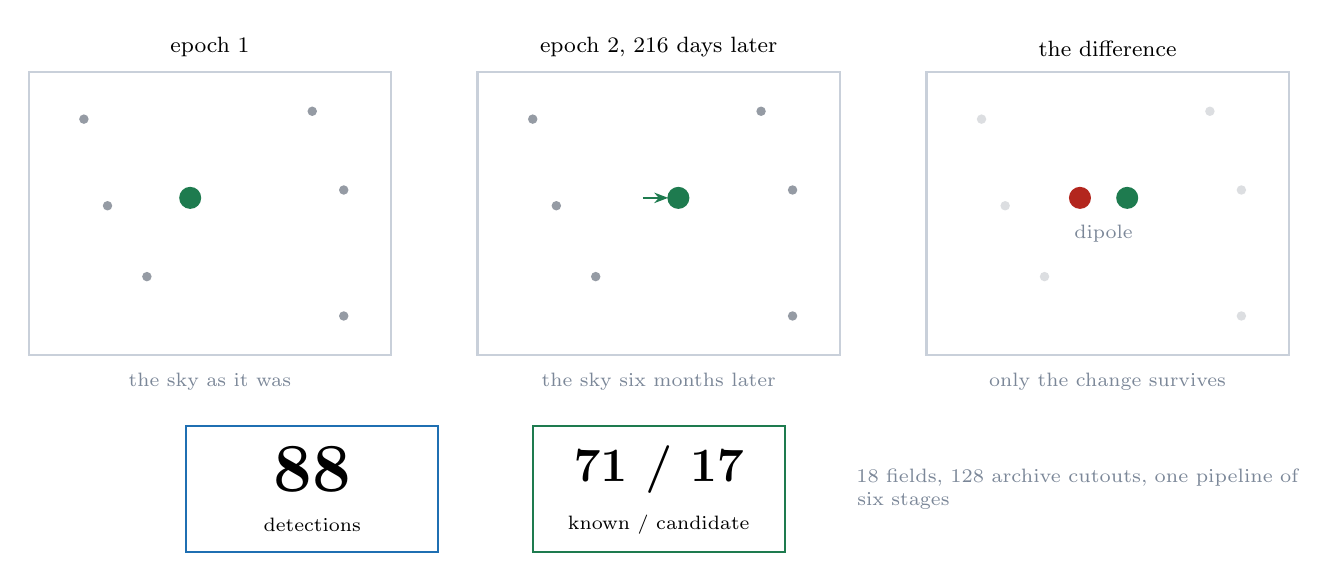
\begin{tikzpicture}[font=\footnotesize]
  % three panels, generous gutters
  \foreach \x/\lab in {0/{epoch 1},5.7/{epoch 2, 216 days later},11.4/{the difference}}{\draw[rule,thick,fill=white] (\x,3.0) rectangle (\x+4.6,6.6); \node[above=2pt] at (\x+2.3,6.6) {\lab};}
  \foreach \x/\y in {0.7/6.0,1.5/4.0,3.6/6.1,4.0/3.5,1.0/4.9,4.0/5.1}{\fill[slate!55] (\x,\y) circle (0.06); \fill[slate!55] (\x+5.7,\y) circle (0.06); \fill[slate!18] (\x+11.4,\y) circle (0.06);}
  % moving source: epoch 1, epoch 2, difference
  \fill[good] (2.05,5.0) circle (0.14);
  \fill[good] (5.7+2.55,5.0) circle (0.14);
  \draw[-{Stealth[length=5pt]},thick,good] (5.7+2.10,5.0) -- (5.7+2.42,5.0);
  \fill[bad] (11.4+1.95,5.0) circle (0.14);
  \fill[good] (11.4+2.55,5.0) circle (0.14);
  \node[anchor=north,font=\scriptsize,text=muted] at (11.4+2.25,4.78) {dipole};
  % captions under each panel, on one line each
  \node[anchor=north,font=\scriptsize,text=muted] at (2.3,2.9) {the sky as it was};
  \node[anchor=north,font=\scriptsize,text=muted] at (5.7+2.3,2.9) {the sky six months later};
  \node[anchor=north,font=\scriptsize,text=muted] at (11.4+2.3,2.9) {only the change survives};
  % hero numbers, own row
  \draw[accent,thick] (2.0,0.5) rectangle (5.2,2.1);
  \node at (3.6,1.55) {\Huge\bfseries 88};
  \node[font=\scriptsize] at (3.6,0.85) {detections};
  \draw[good,thick] (6.4,0.5) rectangle (9.6,2.1);
  \node at (8.0,1.55) {\LARGE\bfseries 71 / 17};
  \node[font=\scriptsize] at (8.0,0.85) {known / candidate};
  \node[anchor=west,font=\scriptsize,text=muted,text width=5.6cm] at (10.4,1.30) {18 fields, 128 archive cutouts, one pipeline of six stages};
\end{tikzpicture}}

\textbf{Spoken script.} Good morning. NASA's SPHEREx satellite photographs the whole sky in a hundred
and two infrared colours, and it does it again roughly every six months. My question is the oldest one
in time-domain astronomy, asked of this new data: looking at two of those photographs of the same patch
of sky, can we say what changed -- and can we be honest about what we cannot tell? Eighteen fields, one
hundred and twenty-eight archive images, eighty-eight detections, of which seventy-one turn out to be
objects that were already catalogued. Most of the next twenty minutes is about how it works and why
each step is built the way it is.

\newpage
% --------------------------------------------------------------- SLIDE 2 ---
\slidehead{2}{Why difference imaging at all}{0:55}

\textbf{On the slide.}
\begin{itemize}[leftmargin=1.4em,itemsep=2pt,topsep=2pt]
\item One image shows what is there; a pair shows what is happening
\item Subtract two visits: the constant sky cancels, the change survives
\item Two shapes of change: a dipole (moved) and a monopole (brightened)
\item A difference image is still not a discovery -- systematics dominate it
\end{itemize}

\textbf{Figure / diagram.} Three large panels -- visit 1, visit 2, the difference -- plus a fourth
small panel for a variable, and a labelled haze for the systematics that survive subtraction.

\figbox{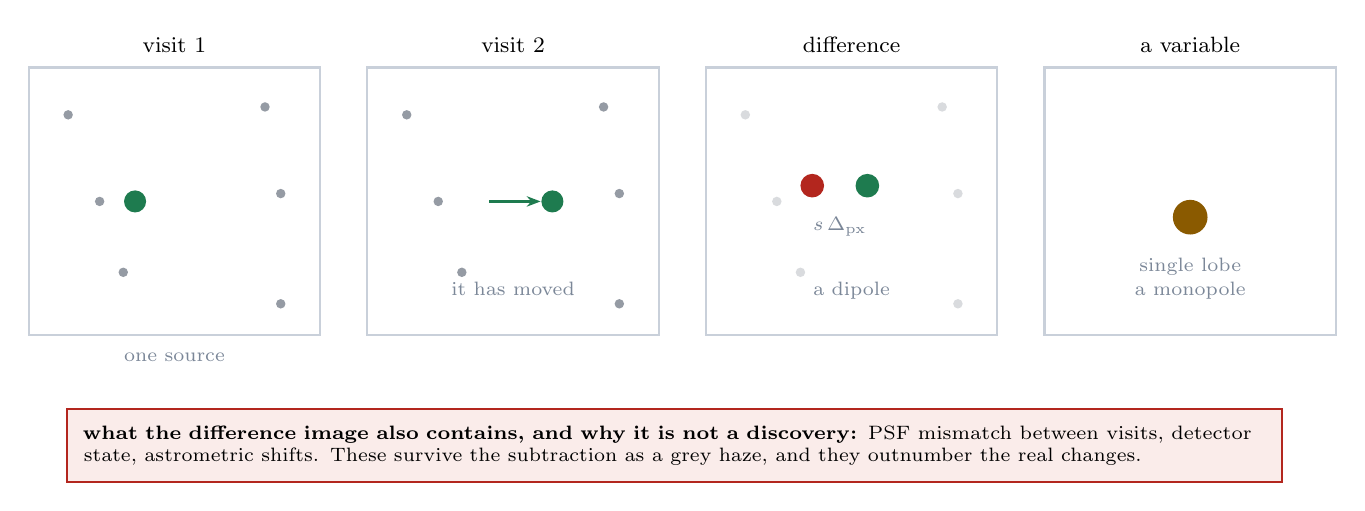
\begin{tikzpicture}[font=\footnotesize]
  \foreach \x/\lab in {0/{visit 1},4.3/{visit 2},8.6/{difference},12.9/{a variable}}{\draw[rule,thick,fill=white] (\x,3.0) rectangle (\x+3.7,6.4); \node[above=2pt] at (\x+1.85,6.4) {\lab};}
  \foreach \x/\y in {0.5/5.8,1.2/3.8,3.0/5.9,3.2/3.4,0.9/4.7,3.2/4.8}{\fill[slate!55] (\x,\y) circle (0.06); \fill[slate!55] (\x+4.3,\y) circle (0.06); \fill[slate!20] (\x+8.6,\y) circle (0.06);}
  \fill[good] (1.35,4.7) circle (0.14);
  \fill[good] (4.3+2.35,4.7) circle (0.14);
  \draw[-{Stealth[length=5pt]},thick,good] (4.3+1.55,4.7) -- (4.3+2.20,4.7);
  \fill[bad] (8.6+1.35,4.9) circle (0.15);
  \fill[good] (8.6+2.05,4.9) circle (0.15);
  \node[anchor=north,font=\scriptsize,text=muted] at (8.6+1.70,4.62) {$s\,\Delta_{\rm px}$};
  \fill[warn] (12.9+1.85,4.5) circle (0.22);
  \node[anchor=north,font=\scriptsize,text=muted] at (12.9+1.85,4.10) {single lobe};
  \node[anchor=north,font=\scriptsize,text=muted] at (1.85,2.9) {one source};
  \node[anchor=north,font=\scriptsize,text=muted] at (4.3+1.85,3.8) {it has moved};
  \node[anchor=north,font=\scriptsize,text=muted] at (8.6+1.85,3.8) {a dipole};
  \node[anchor=north,font=\scriptsize,text=muted] at (12.9+1.85,3.8) {a monopole};
  % the haze note, its own row
  \node[draw=bad,thick,fill=bad2,align=left,inner sep=6pt,text width=15.0cm,font=\scriptsize] at (8.2,1.6)
    {\textbf{what the difference image also contains, and why it is not a discovery:} PSF mismatch between visits, detector state, astrometric shifts. These survive the subtraction as a grey haze, and they outnumber the real changes.};
\end{tikzpicture}}

\textbf{Spoken script.} Why bother with the second photograph at all? Because a single image tells you
what is there, and a pair tells you what is happening. Take the same patch of sky, subtract one visit
from the other, and the constant sky cancels to grey. What survives is change, and change has a shape.
If a star moved you get a positive lobe where it is now and a negative lobe where it was: a dipole, and
the separation divided by the time baseline is a proper motion. If a star simply brightened you get one
lobe: a monopole.\par
That is the whole physics, and it is fifty years old. The reason this is still a research problem is
the grey haze labelled under the third panel: what survives subtraction is dominated by the point-spread
function changing between visits, by the detector warming up, by the astrometric solution shifting.
Almost none of those pixels are sky. So the work is not the subtraction -- it is deciding which of
those blobs you are allowed to believe.

\newpage
% --------------------------------------------------------------- SLIDE 3 ---
\slidehead{3}{The problem statement}{1:00}

\textbf{On the slide.}
\begin{itemize}[leftmargin=1.4em,itemsep=2pt,topsep=2pt]
\item Input: two visits to a 9\arcmin{} field, each with a variance plane and a quality bitmask
\item Output: the set $\mathcal{C}=\{\mathbf{x}:|S(\mathbf{x})|>\tau\}$, with a position, a significance,
      a morphology and an \emph{identity verdict}
\item Constraints: public data only; every number reproducible; ``no change'' must be distinguishable
      from ``no data''; laptop scale
\end{itemize}

\textbf{Figure / diagram.} A left-to-right flow in set notation: 32\,400 pixels, a threshold, the 88
detections, then the triage split into 71 known and 17 candidate, with the four constraints in a box
underneath.

\figbox{\begin{tikzpicture}[font=\footnotesize,
  bx/.style={draw=accent,thick,fill=accent2,align=center,inner sep=5pt,text width=3.0cm},
  kn/.style={draw=good,thick,fill=good2,align=center,inner sep=5pt,text width=3.0cm},
  ca/.style={draw=warn,thick,fill=warn2,align=center,inner sep=5pt,text width=3.0cm},
  ar/.style={-{Stealth[length=6pt]},thick,draw=slate}]
  \node[bx] (pix) at (1.5,2.6) {$180\times180$ pixels\\$32\,400$ values of $|S|$};
  \node[bx] (thr) at (6.1,2.6) {threshold\\$|S|>5\sigma$};
  \node[bx] (set) at (10.7,2.6) {$\mathcal{C}$: 88 detections};
  \node[kn] (known) at (15.4,3.6) {71 KNOWN\\a catalogue match};
  \node[ca] (cand) at (15.4,1.6) {17 CANDIDATE\\unexplained};
  \draw[ar] (pix) -- (thr);
  \draw[ar] (thr) -- (set);
  \draw[ar] (set.east) -- ++(0.6,0) |- (known.west);
  \draw[ar] (set.east) -- ++(0.6,0) |- (cand.west);
  \node[draw=bad,thick,fill=bad2,align=left,inner sep=6pt,text width=9.4cm,font=\small] at (5.7,0.05)
    {\textbf{Constraints}\\
     public archive products only \;\textbullet\; every number reproducible from a stored parameter set\\
     ``no change'' $\neq$ ``no data'' \;\textbullet\; it has to run on one laptop};
\end{tikzpicture}}

\textbf{Spoken script.} Let me state the problem precisely, because the precision is the point. Input:
two visits to a nine-arcminute field, each with a variance plane and a quality bitmask. Task: build a
statistic, threshold it, and so obtain the set of sky positions where the flux distribution changed --
that is the set C on the slide -- and attach to each element four things: a sky coordinate, a
significance, a morphology, and an identity verdict. Identity is not optional, because a blob is only
interesting if no catalogue already explains it.\par
Four constraints shaped every design decision. Only public archive products. Every number reproducible
from a stored parameter set. The system must distinguish ``no change'' from ``no data'' -- that sounds
trivial, and it is the single most common failure in this kind of pipeline. And the whole thing has to
run on a laptop. The numbers follow from that: thirty-two thousand pixels in, eighty-eight detections
out, seventy-one explained, seventeen not.

\newpage
% --------------------------------------------------------------- SLIDE 4 ---
\slidehead{4}{Focus and research questions}{0:45}

\textbf{On the slide.}
\begin{itemize}[leftmargin=1.4em,itemsep=2pt,topsep=2pt]
\item RQ1: is the significance map calibrated on co-added SPHEREx images?
\item RQ2: does dipole/monopole morphology separate movers from variables at 3\arcsec{} sampling?
\item RQ3: how much of the candidate list do Gaia, WISE and VSX explain away?
\item RQ4: what does injection--recovery say -- and if it says ``nothing'', how is that reported?
\end{itemize}

\textbf{Figure / diagram.} Four numbered question cards in a row, each with its one-line answer
status underneath, and a footer strip listing what is explicitly out of scope.

\figbox{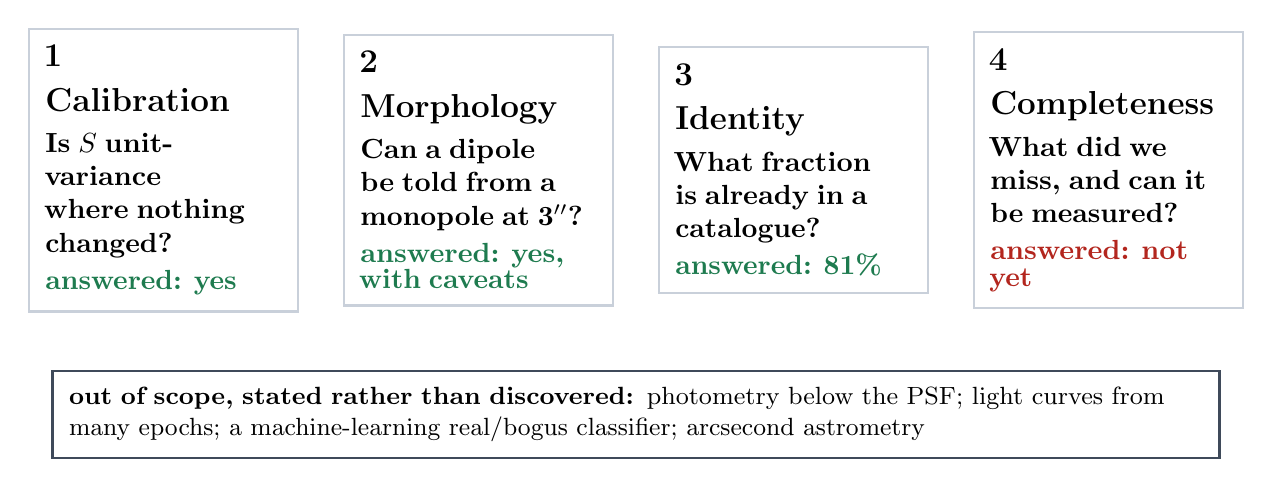
\begin{tikzpicture}[font=\footnotesize,
  card/.style={draw=rule,thick,fill=white,align=left,inner sep=6pt,text width=3.0cm}]
  \node[card] (a) at (2.0,4.6) {\large\bfseries 1\par\vspace{2pt}Calibration\par\vspace{3pt}\normalsize Is $S$ unit-variance where nothing changed?\par\vspace{4pt}\textcolor{good}{\bfseries answered: yes}};
  \node[card] (b) at (6.0,4.6) {\large\bfseries 2\par\vspace{2pt}Morphology\par\vspace{3pt}\normalsize Can a dipole be told from a monopole at 3\arcsec?\par\vspace{4pt}\textcolor{good}{\bfseries answered: yes, with caveats}};
  \node[card] (c) at (10.0,4.6) {\large\bfseries 3\par\vspace{2pt}Identity\par\vspace{3pt}\normalsize What fraction is already in a catalogue?\par\vspace{4pt}\textcolor{good}{\bfseries answered: 81\%}};
  \node[card] (d) at (14.0,4.6) {\large\bfseries 4\par\vspace{2pt}Completeness\par\vspace{3pt}\normalsize What did we miss, and can it be measured?\par\vspace{4pt}\textcolor{bad}{\bfseries answered: not yet}};
  \node[draw=slate,thick,fill=white,align=left,inner sep=6pt,text width=14.4cm,font=\small] at (8.0,1.5)
    {\textbf{out of scope, stated rather than discovered:} photometry below the PSF; light curves from many epochs; a machine-learning real/bogus classifier; arcsecond astrometry};
\end{tikzpicture}}

\textbf{Spoken script.} I want to be explicit about what is and is not in scope, because a small project
like this either draws its boundary honestly or it oversells. Four questions, and the answers are on the
cards. One: is the statistic actually calibrated, so that five sigma means what it says. Two: can the
morphology test tell a moved star from a flickering one at three-arcsecond sampling. Three: how much of
the candidate list is already in Gaia, WISE or the variable-star index -- the question that decides
whether anything here is interesting. Four: what did we miss, and here the honest answer is ``not yet
known'', which I will come back to on slide seventeen.\par
And the footer strip is deliberate: no PSF-level photometry, no light curves, no machine-learning
real/bogus classifier, no arcsecond astrometry. Stated up front rather than discovered by a reviewer.

\newpage

% --------------------------------------------------------------- SLIDE 5 ---
\slidehead{5}{Prior art I: the subtraction lineage}{1:00}

\textbf{On the slide.}
\begin{itemize}[leftmargin=1.4em,itemsep=2pt,topsep=2pt]
\item 1998 Alard \& Lupton: fit a convolution kernel so that both images share a PSF (ISM)
\item 2008 Bramich: a discrete per-pixel kernel, well posed in sparse fields
\item 2016 ZOGY: no fitting at all; the optimal difference and a unit-variance significance map
\item 2022 SFFT: the same mathematics, better behaved for undersampled space PSFs
\end{itemize}

\textbf{Figure / diagram.} A timeline with the four milestones, and under two of them a small sketch
contrasting ``fit until the curves agree'' with ``convolve both to a common PSF''.

\figbox{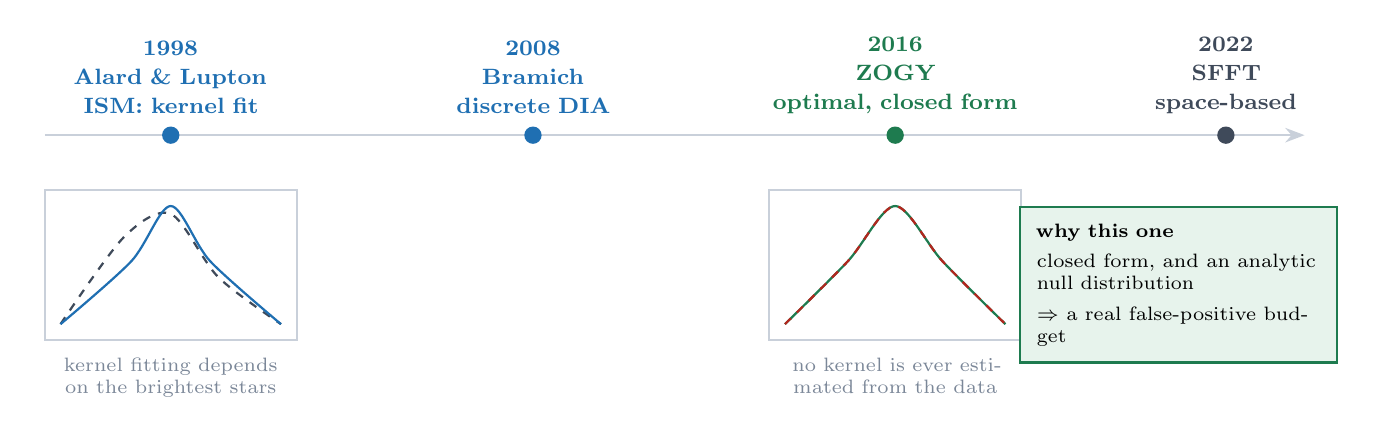
\begin{tikzpicture}[font=\footnotesize]
  \draw[-{Stealth[length=7pt]},thick,rule] (0.2,4.9) -- (16.2,4.9);
  \foreach \x/\yr/\la/\lb/\col in {
    1.8/1998/{Alard \& Lupton}/{ISM: kernel fit}/accent,
    6.4/2008/{Bramich}/{discrete DIA}/accent,
    11.0/2016/{ZOGY}/{optimal, closed form}/good,
    15.2/2022/{SFFT}/{space-based}/slate}{
    \fill[\col] (\x,4.9) circle (0.11);
    \node[anchor=south,text=\col,align=center,text width=3.4cm] at (\x,5.05) {\bfseries \yr\\[1pt] \la\\[1pt] \lb};}
  % sketch one: kernel fit
  \draw[rule,thick,fill=white] (0.2,2.3) rectangle (3.4,4.2);
  \draw[slate,dashed,thick] plot[smooth] coordinates {(0.4,2.5) (1.2,3.6) (1.8,3.9) (2.4,3.1) (3.2,2.5)};
  \draw[accent,thick] plot[smooth] coordinates {(0.4,2.5) (1.3,3.3) (1.8,4.0) (2.3,3.3) (3.2,2.5)};
  \node[anchor=north,font=\scriptsize,text=muted,text width=3.2cm,align=center] at (1.8,2.2) {kernel fitting depends on the brightest stars};
  % sketch two: proper subtraction
  \draw[rule,thick,fill=white] (9.4,2.3) rectangle (12.6,4.2);
  \draw[good,thick] plot[smooth] coordinates {(9.6,2.5) (10.4,3.3) (11.0,4.0) (11.6,3.3) (12.4,2.5)};
  \draw[bad,thick,dashed] plot[smooth] coordinates {(9.6,2.5) (10.4,3.3) (11.0,4.0) (11.6,3.3) (12.4,2.5)};
  \node[anchor=north,font=\scriptsize,text=muted,text width=3.2cm,align=center] at (11.0,2.2) {no kernel is ever estimated from the data};
  % why this one
  \node[draw=good,thick,fill=good2,align=left,inner sep=6pt,text width=3.6cm,font=\scriptsize] at (14.6,3.0)
    {\textbf{why this one}\\[3pt] closed form, and an analytic null distribution\\[3pt] $\Rightarrow$ a real false-positive budget};
\end{tikzpicture}}

\textbf{Spoken script.} Subtraction was solved in stages, and the stages matter for what I could assume.
In 1998 Alard and Lupton fitted a convolution kernel that maps one image onto the other so that both end
up with the same point-spread function -- that is what made the microlensing surveys possible. It works,
but the fit is dominated by the brightest stars in the field, which is exactly what you cannot rely on in
a nebula or a crowded field. In 2008 Bramich made the kernel per-pixel and well posed in sparse fields;
you trade noise for stability.\par
Then in 2016 Zackay, Ofek and Gal-Yam did something conceptually different: instead of fitting anything
they derived the statistically optimal difference image in Fourier space, and with it a significance map
with unit variance by construction wherever the sky did not change. SFFT in 2022 is the modern
reformulation and it is what Rubin will use. I chose ZOGY for the reason on the right of this slide:
because the null distribution is analytic, the false-positive budget can be computed rather than
measured, and that is what lets me defend a five-sigma threshold later.

\newpage
% --------------------------------------------------------------- SLIDE 6 ---
\slidehead{6}{Prior art II: brokers, and the gap this fills}{0:55}

\textbf{On the slide.}
\begin{itemize}[leftmargin=1.4em,itemsep=2pt,topsep=2pt]
\item Every operational survey runs the same four ideas: template, subtract, veto, triage
\item Brokers (ANTARES, ALeRCE, Lasair, Fink) industrialise the veto with machine learning
\item For SPHEREx there is no published open end-to-end difference-imaging artefact
\item The gap is not an algorithm -- it is an inspectable, reproducible instance
\end{itemize}

\textbf{Figure / diagram.} The detect--veto--human loop on the left, and on the right a bar chart of
how much of those four ideas each body of work actually ships as something a reader can open.

\figbox{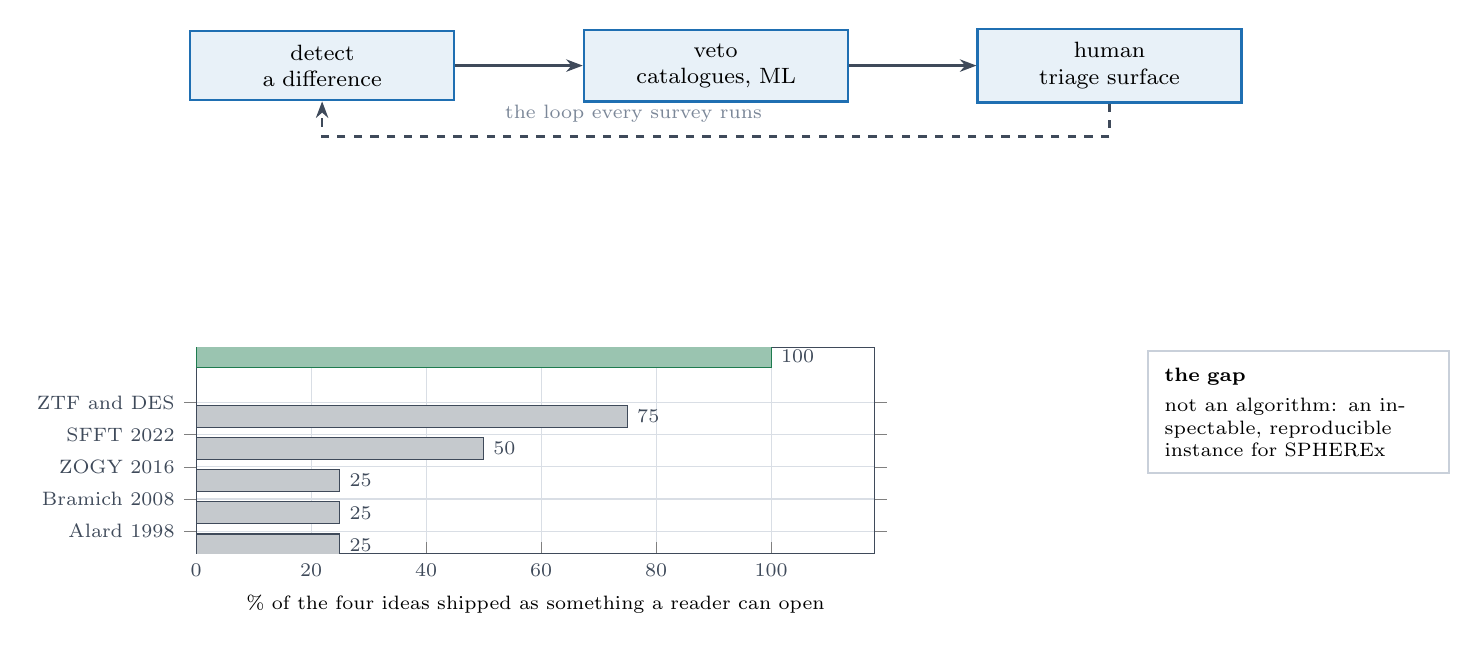
\begin{tikzpicture}[font=\footnotesize,
  n/.style={draw=accent,thick,fill=accent2,align=center,inner sep=5pt,text width=3.0cm},
  ar/.style={-{Stealth[length=6pt]},draw=slate,thick}]
  \node[n] (d) at (2.0,6.4) {detect\\a difference};
  \node[n] (v) at (7.0,6.4) {veto\\catalogues, ML};
  \node[n] (h) at (12.0,6.4) {human\\triage surface};
  \draw[ar] (d) -- (v);
  \draw[ar] (v) -- (h);
  \draw[ar,dashed] (h.south) -- (12.0,5.5) -- (2.0,5.5) -- (d.south);
  \node[font=\scriptsize,text=muted,anchor=south west] at (4.2,5.56) {the loop every survey runs};
  \begin{scope}[shift={(0.4,0.2)}]
    \begin{axis}[width=10.2cm,height=4.2cm,xbar,bar width=8pt,xmin=0,xmax=118,
      xlabel={\% of the four ideas shipped as something a reader can open},xlabel style={font=\scriptsize},
      symbolic y coords={{Alard 1998},{Bramich 2008},{ZOGY 2016},{SFFT 2022},{ZTF and DES},{this work}},
      ytick=data,tick label style={font=\scriptsize,text=slate},axis line style={slate},
      grid=major,grid style={rule!70},nodes near coords,nodes near coords style={font=\scriptsize,text=slate},
      enlarge y limits=0.14]
    \addplot[fill=slate!30,draw=slate] coordinates {(25,{Alard 1998}) (25,{Bramich 2008}) (25,{ZOGY 2016}) (50,{SFFT 2022}) (75,{ZTF and DES})};
    \addplot[fill=good!45,draw=good] coordinates {(100,{this work})};
    \end{axis}
  \end{scope}
  \node[draw=rule,thick,fill=white,align=left,inner sep=6pt,text width=3.4cm,font=\scriptsize] at (14.4,2.0)
    {\textbf{the gap}\\[3pt] not an algorithm: an inspectable, reproducible instance for SPHEREx};
\end{tikzpicture}}

\textbf{Spoken script.} Everything since the 1990s runs the same loop, and it is worth naming as a loop:
you detect against a template, you veto with catalogues and increasingly with machine learning, and you
put what survives in front of a human. The big surveys industrialised each step -- ZTF, ATLAS, DES, and
now Rubin, with brokers called ANTARES, ALeRCE, Lasair and Fink doing the vetting. They are enormously
more capable than anything I built.\par
So the gap is not algorithmic. The bars on the right are my own assessment of how much of that
four-part pattern each line of work ships as something a reader can actually inspect: the classical
papers give equations and sometimes a reference code; the surveys give a pipeline you cannot open; the
brokers give a service. What does not exist, as far as I could find, is a small end-to-end artefact for
SPHEREx specifically, where you can follow one pixel from a NASA archive file to a verdict on a web
page, including the parts that fail. That is what this is.

\newpage

% --------------------------------------------------------------- SLIDE 7 ---
\slidehead{7}{SPHEREx: the instrument and the data products}{0:55}

\textbf{On the slide.}
\begin{itemize}[leftmargin=1.4em,itemsep=2pt,topsep=2pt]
\item One telescope, six detectors, 102 bands from 0.75 to 5.0\,\textmu m
\item Level-2 products are small spectral images: every pixel carries a wavelength
\item Four extensions: IMAGE, VAR, FLAGS (32 bits), and WCS-WAVE $(x,y,\lambda)$
\item Six-month cadence $\Rightarrow$ what survives subtraction is astrophysical, not asteroids
\end{itemize}

\textbf{Figure / diagram.} The six-detector focal plane above a wavelength axis with the bands actually
used highlighted, and the three extensions that make difference imaging possible underneath.

\figbox{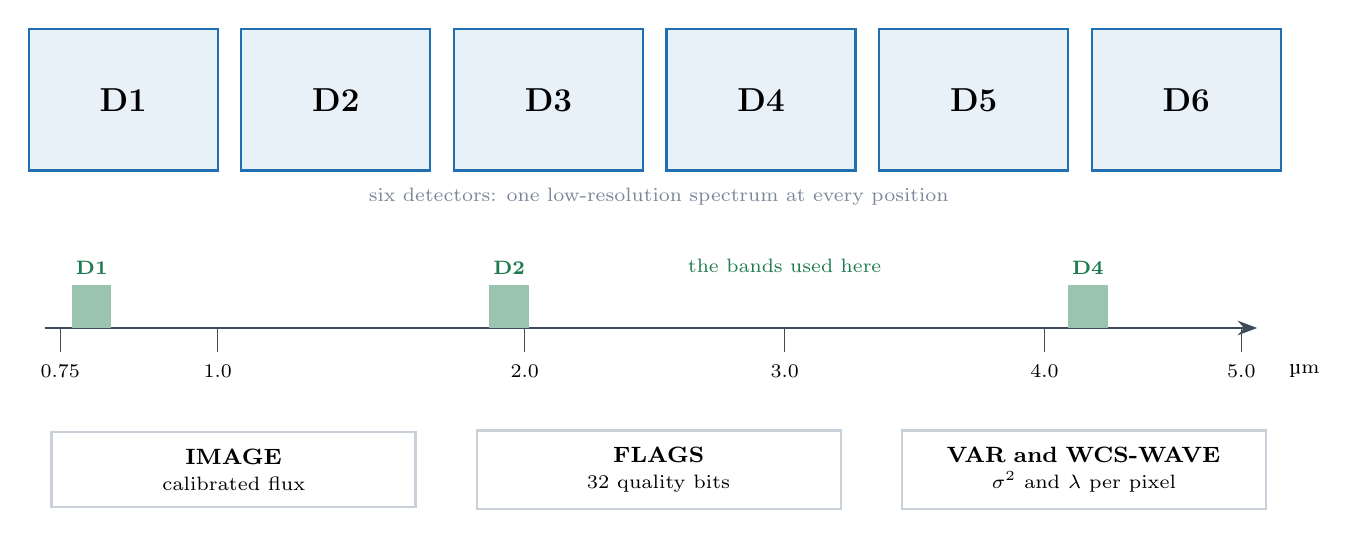
\begin{tikzpicture}[font=\footnotesize]
  \foreach \lab/\x in {D1/0,D2/2.7,D3/5.4,D4/8.1,D5/10.8,D6/13.5}{\draw[accent,thick,fill=accent2] (\x,5.4) rectangle (\x+2.4,7.2); \node at (\x+1.2,6.3) {\large\bfseries \lab};}
  \node[anchor=north,font=\scriptsize,text=muted] at (8.0,5.3) {six detectors: one low-resolution spectrum at every position};
  \draw[-{Stealth[length=7pt]},thick,slate] (0.2,3.4) -- (15.6,3.4);
  \foreach \w/\x in {0.75/0.4,1.0/2.4,2.0/6.3,3.0/9.6,4.0/12.9,5.0/15.4}{\draw[slate] (\x,3.4) -- (\x,3.1); \node[anchor=north,font=\scriptsize] at (\x,3.05) {\w};}
  \node[anchor=north,font=\scriptsize] at (16.2,3.05) {\textmu m};
  \fill[good!45] (0.55,3.4) rectangle (1.05,3.95); \node[anchor=south,font=\scriptsize\bfseries,text=good] at (0.8,3.95) {D1};
  \fill[good!45] (5.85,3.4) rectangle (6.35,3.95); \node[anchor=south,font=\scriptsize\bfseries,text=good] at (6.1,3.95) {D2};
  \fill[good!45] (13.2,3.4) rectangle (13.7,3.95); \node[anchor=south,font=\scriptsize\bfseries,text=good] at (13.45,3.95) {D4};
  \node[anchor=south,font=\scriptsize,text=good] at (9.6,3.98) {the bands used here};
  \node[draw=rule,thick,fill=white,align=center,inner sep=6pt,text width=4.2cm] at (2.6,1.6) {\textbf{IMAGE}\\ \scriptsize calibrated flux};
  \node[draw=rule,thick,fill=white,align=center,inner sep=6pt,text width=4.2cm] at (8.0,1.6) {\textbf{FLAGS}\\ \scriptsize 32 quality bits};
  \node[draw=rule,thick,fill=white,align=center,inner sep=6pt,text width=4.2cm] at (13.4,1.6) {\textbf{VAR and WCS-WAVE}\\ \scriptsize $\sigma^2$ and $\lambda$ per pixel};
\end{tikzpicture}}

\textbf{Spoken script.} A word on the instrument, because the shape of the data drives everything
downstream. SPHEREx is a small telescope with six detectors that sweeps the sky and, unusually, takes a
low-resolution spectrum at every position: a hundred and two bands between zero-point-seven-five and
five microns. So the Level-2 product is not a broadband picture, it is a little spectral image, and each
file carries four things I care about: the calibrated image, the variance, a thirty-two-bit quality
mask, and a table giving the wavelength of every pixel.\par
Two consequences. First, the cadence is about six months, so anything that moved fast -- an asteroid,
say -- has left the field entirely; what survives subtraction is genuine variability or genuine high
proper motion. Second, because every pixel knows its wavelength, a detection can be diagnosed
spectrally with no follow-up telescope, which is what slide sixteen is about.

\newpage
% --------------------------------------------------------------- SLIDE 8 ---
\slidehead{8}{The archive mechanics, and the eighteen fields}{0:55}

\textbf{On the slide.}
\begin{itemize}[leftmargin=1.4em,itemsep=2pt,topsep=2pt]
\item Two calls: a SIA2 cone search (cached as a VOTable), then the cutout service
\item 5.3\,MB sections of a 70\,MB parent frame -- this is what makes the project feasible
\item Acceptance: $\ge$12\,px margin inside the cutout, and under 50\% of pixels flagged
\item 18 fields, 128 cutouts, 0.88\,GB; the Large Magellanic Cloud was tried and dropped
\end{itemize}

\textbf{Figure / diagram.} Left: the sky distribution of all eighteen fields. Right: the two-step
fetch path with its cost annotated, and the acceptance test at the end.

\figbox{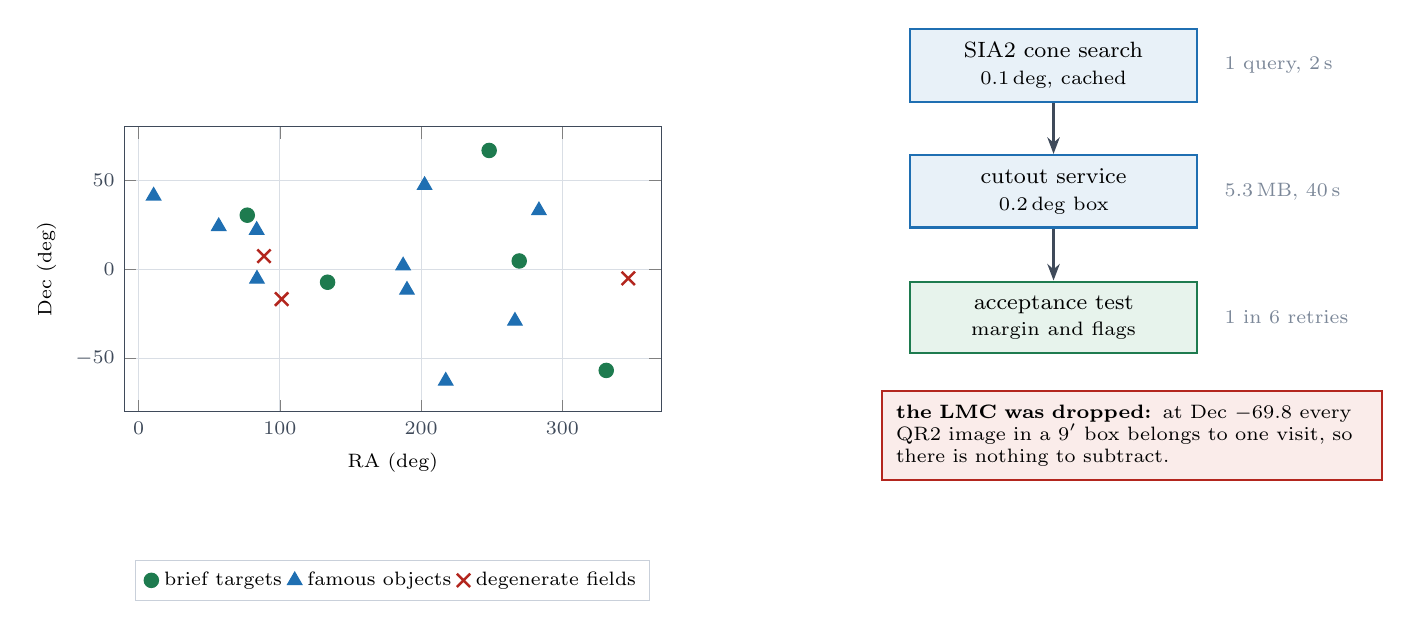
\begin{tikzpicture}[font=\footnotesize]
  \begin{scope}
    \begin{axis}[width=8.4cm,height=5.2cm,
      xlabel={RA (deg)},ylabel={Dec (deg)},xmin=-10,xmax=370,ymin=-80,ymax=80,
      xlabel style={font=\scriptsize},ylabel style={font=\scriptsize},
      grid=both,grid style={rule!70},axis line style={slate},
      tick label style={font=\scriptsize,text=slate},
      legend style={font=\scriptsize,draw=rule,at={(0.5,-0.52)},anchor=north,legend columns=3}]
    \addplot[only marks,mark=*,mark size=2.6pt,good] coordinates {
      (269.45,4.69) (331.04,-56.78) (76.96,30.40) (248.17,66.75) (133.80,-7.25)};
    \addlegendentry{brief targets}
    \addplot[only marks,mark=triangle*,mark size=3.0pt,accent] coordinates {
      (10.68,41.27) (83.82,-5.39) (56.75,24.12) (83.63,22.01) (202.47,47.20) (190.00,-11.62)
      (283.40,33.03) (266.42,-29.01) (187.28,2.05) (217.43,-62.68)};
    \addlegendentry{famous objects}
    \addplot[only marks,mark=x,mark size=3.4pt,bad,line width=0.9pt] coordinates {
      (88.79,7.41) (101.29,-16.72) (346.62,-5.04)};
    \addlegendentry{degenerate fields}
    \end{axis}
  \end{scope}
  % fetch path on the right
  \begin{scope}[shift={(9.9,0.2)}]
    \node[draw=accent,thick,fill=accent2,align=center,inner sep=5pt,text width=3.3cm] (a) at (1.9,4.2)
      {SIA2 cone search\\ \scriptsize 0.1\,deg, cached};
    \node[draw=accent,thick,fill=accent2,align=center,inner sep=5pt,text width=3.3cm] (b) at (1.9,2.6)
      {cutout service\\ \scriptsize 0.2\,deg box};
    \node[draw=good,thick,fill=good2,align=center,inner sep=5pt,text width=3.3cm] (c) at (1.9,1.0)
      {acceptance test\\ \scriptsize margin and flags};
    \draw[-{Stealth[length=6pt]},thick,slate] (a) -- (b);
    \draw[-{Stealth[length=6pt]},thick,slate] (b) -- (c);
    \node[right,font=\scriptsize,text=muted,align=left] at (3.95,4.2) {1 query, 2\,s};
    \node[right,font=\scriptsize,text=muted,align=left] at (3.95,2.6) {5.3\,MB, 40\,s};
    \node[right,font=\scriptsize,text=muted,align=left] at (3.95,1.0) {1 in 6 retries};
    \node[draw=bad,thick,fill=bad2,align=left,inner sep=5pt,text width=6.0cm,font=\scriptsize] at (2.9,-0.5)
      {\textbf{the LMC was dropped:} at Dec $-69.8$ every QR2 image in a 9\arcmin{} box belongs to one visit, so there is nothing to subtract.};
  \end{scope}
\end{tikzpicture}}

\textbf{Spoken script.} Getting the data takes exactly two archive calls, and I want to show them
because the cost shapes the design. First a SIA2 cone search: give it a position and it returns every
Level-2 image whose footprint covers it. That answer is cached verbatim, so re-running never asks again.
Then the cutout service, which is the trick that makes this possible: instead of downloading
seventy-megabyte parents, I ask for a five-megabyte section around my target. Even so a cutout takes
about forty seconds at the archive's throttled rate, and roughly one request in six times out and has
to fall back -- hence the acceptance test at the bottom of that column.\par
The map shows the eighteen fields: five chosen by the brief -- two high-proper-motion stars, two
variables, one extreme cool dwarf -- and thirteen I added, galaxies and nebulae and a quasar, to prove
the pipeline is not tuned to one kind of object. One object, the Large Magellanic Cloud, I tried and
dropped, for the reason in the red box. That is on the record rather than quietly removed.

\newpage
% --------------------------------------------------------------- SLIDE 9 ---
\slidehead{9}{Architecture: six stages, one cache}{0:55}

\textbf{On the slide.}
\begin{itemize}[leftmargin=1.4em,itemsep=2pt,topsep=2pt]
\item Ingest, co-add, subtract, triage, diagnose, validate
\item Each stage is a file with its own entry point: the chain can be entered anywhere
\item One metadata file per field is the contract between stages
\item The serving layer is separate: it calls stages two to five, or reads pre-rendered JSON
\end{itemize}

\textbf{Figure / diagram.} The six stages in two rows, the on-disk cache under the first, and the
serving layer at the bottom, with the line count of each module written inside its box.

\figbox{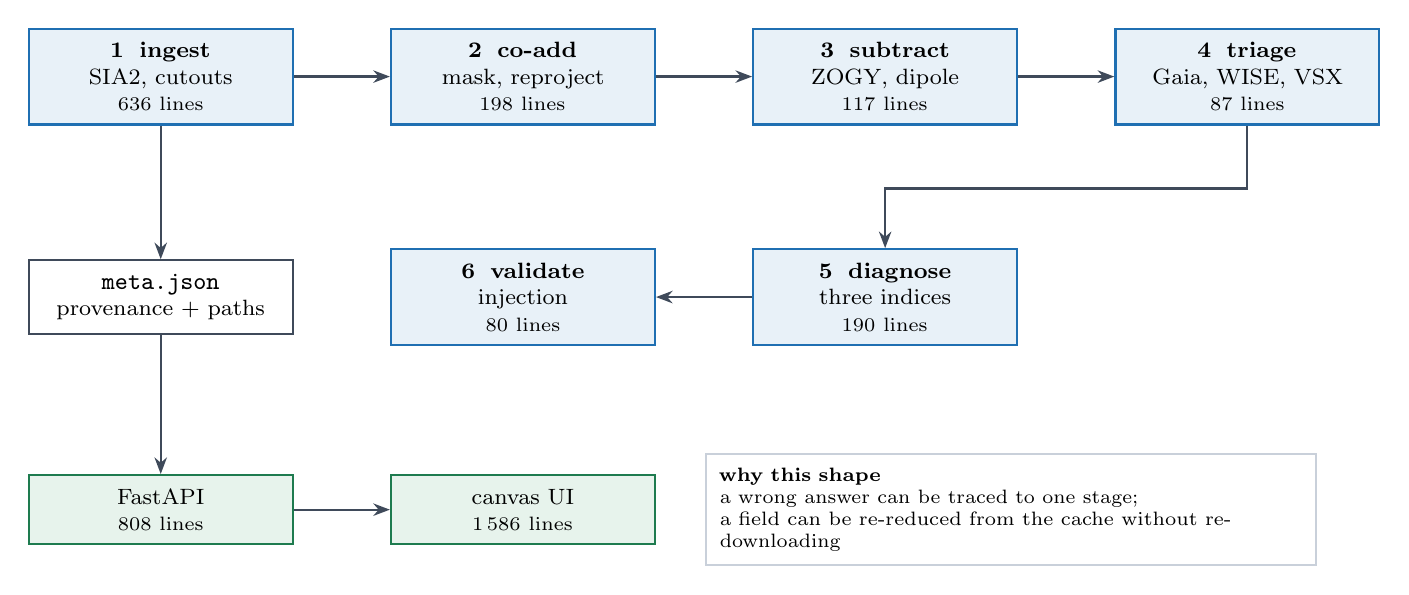
\begin{tikzpicture}[font=\footnotesize,node distance=6mm and 7mm,
  b/.style={draw=accent,thick,fill=accent2,align=center,inner sep=5pt,text width=3.0cm},
  c/.style={draw=slate,thick,fill=white,align=center,inner sep=5pt,text width=3.0cm},
  s/.style={draw=good,thick,fill=good2,align=center,inner sep=5pt,text width=3.0cm},
  ar/.style={-{Stealth[length=6pt]},thick,draw=slate}]
  \node[b] (s1) at (1.6,6.2) {\textbf{1\; ingest}\\ SIA2, cutouts\\ \scriptsize 636 lines};
  \node[b] (s2) at (6.2,6.2) {\textbf{2\; co-add}\\ mask, reproject\\ \scriptsize 198 lines};
  \node[b] (s3) at (10.8,6.2) {\textbf{3\; subtract}\\ ZOGY, dipole\\ \scriptsize 117 lines};
  \node[b] (s4) at (15.4,6.2) {\textbf{4\; triage}\\ Gaia, WISE, VSX\\ \scriptsize 87 lines};
  \node[b] (s5) at (10.8,3.4) {\textbf{5\; diagnose}\\ three indices\\ \scriptsize 190 lines};
  \node[b] (s6) at (6.2,3.4) {\textbf{6\; validate}\\ injection\\ \scriptsize 80 lines};
  \draw[ar] (s1) -- (s2); \draw[ar] (s2) -- (s3); \draw[ar] (s3) -- (s4);
  \draw[ar] (s4.south) -- ++(0,-0.8) -| (s5.north);
  \draw[ar] (s5) -- (s6);
  \node[c] (cache) at (1.6,3.4) {\code{meta.json}\\ provenance + paths};
  \draw[ar] (s1) -- (cache);
  \node[s] (api) at (1.6,0.7) {FastAPI\\ \scriptsize 808 lines};
  \node[s] (ui) at (6.2,0.7) {canvas UI\\ \scriptsize 1\,586 lines};
  \draw[ar] (cache) -- (api);
  \draw[ar] (api) -- (ui);
  \node[draw=rule,thick,fill=white,align=left,inner sep=5pt,text width=7.4cm,font=\scriptsize] at (12.4,0.7)
    {\textbf{why this shape}\\ a wrong answer can be traced to one stage;\\ a field can be re-reduced from the cache without re-downloading};
\end{tikzpicture}}

\textbf{Spoken script.} Six stages, and each is a separate file with its own entry point, which matters
more than it sounds: when something looks wrong I can re-run one stage on cached data instead of the
whole chain. Stage one talks to the archive and writes a metadata file. That file is the contract --
every later stage reads it and nothing else, so the chain is deterministic and restartable. Stage two
masks and combines, stage three subtracts, stage four triages against catalogues, stage five measures a
spectrum and three indices, stage six is the validation.\par
Underneath sits the serving layer: a service that either runs stages two to five on demand or, for the
deployed site, reads pre-rendered JSON for exactly the same responses. That separation is what lets the
same page work with or without a server, which is slide nineteen.

\newpage
% -------------------------------------------------------------- SLIDE 10 ---
\slidehead{10}{Theory I: masking, then an inverse-variance co-add}{0:55}

\textbf{On the slide.}
\begin{itemize}[leftmargin=1.4em,itemsep=2pt,topsep=2pt]
\item Sixteen FLAGS classes are rejected: SUR transients, overflow, phantom, edge, hot/cold, persistence
\item Two are kept: ``full sample'' (informational) and ``source'' (real flux, not a defect)
\item $C=\sum_k w_k\tilde I_k/\sum_k w_k$ with $w_k=1/\tilde V_k$, so $\sigma^2_C=(\sum_k w_k)^{-1}$
\item Honest masking changes the median noise by about a factor of two on the worst frames
\end{itemize}

\textbf{Figure / diagram.} Left: the flag census for the dominant bit classes. Right: a pixel grid
showing which cells survive masking, with the weighting formula beside it.

\figbox{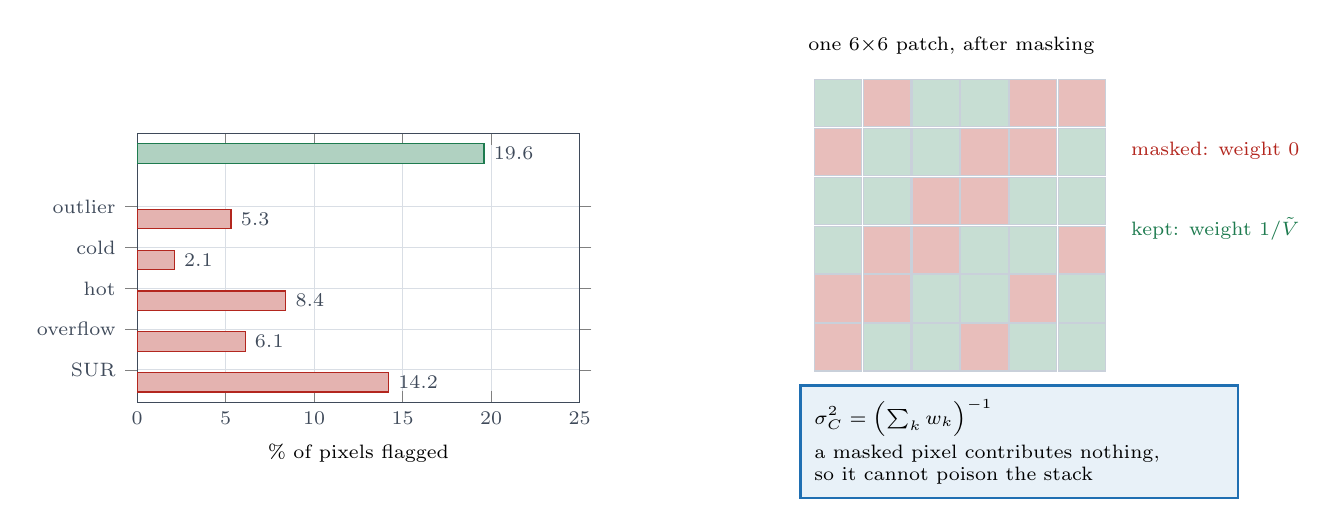
\begin{tikzpicture}[font=\footnotesize]
  \begin{scope}
    \begin{axis}[width=7.2cm,height=5.0cm,xbar,bar width=7pt,xmin=0,xmax=25,
      xlabel={\% of pixels flagged},xlabel style={font=\scriptsize},
      symbolic y coords={{SUR},{overflow},{hot},{cold},{outlier},{source}},
      ytick=data,tick label style={font=\scriptsize,text=slate},axis line style={slate},
      grid=major,grid style={rule!70},nodes near coords,nodes near coords style={font=\scriptsize,text=slate},
      enlarge y limits=0.16]
    \addplot[fill=bad!35,draw=bad] coordinates {(14.2,{SUR}) (6.1,{overflow}) (8.4,{hot}) (2.1,{cold}) (5.3,{outlier})};
    \addplot[fill=good!35,draw=good] coordinates {(19.6,{source})};
    \end{axis}
  \end{scope}
  % pixel grid
  \begin{scope}[shift={(8.6,0.4)}]
    \node[anchor=south west,font=\scriptsize] at (-0.2,3.9) {one 6$\times$6 patch, after masking};
    \foreach \i in {0,...,5}{\foreach \j in {0,...,5}{
      \pgfmathsetmacro{\m}{int(mod(\i*7+\j*3,10))}
      \ifnum\m<4 \def\cc{bad!30}\else\def\cc{good!25}\fi
      \draw[rule,fill=\cc] (\i*0.62,\j*0.62) rectangle (\i*0.62+0.6,\j*0.62+0.6);}}
    \node[font=\scriptsize,text=bad,anchor=west] at (3.9,2.8) {masked: weight 0};
    \node[font=\scriptsize,text=good,anchor=west] at (3.9,1.8) {kept: weight $1/\tilde V$};
    \node[draw=accent,thick,fill=accent2,align=left,inner sep=5pt,text width=5.2cm,font=\scriptsize] at (2.6,-0.9)
      {$\sigma^2_C=\Bigl(\sum_k w_k\Bigr)^{-1}$\\[2pt] a masked pixel contributes nothing,\\ so it cannot poison the stack};
  \end{scope}
\end{tikzpicture}}

\textbf{Spoken script.} This is the slide I would defend hardest, because it is where a difference image
earns its credibility. Every SPHEREx pixel arrives with a variance and a set of quality bits, and most of
those bits mean ``do not trust this pixel''. If you average them in anyway, a handful of cosmic rays and
hot pixels inflate your noise and you silently lose the faint end. So sixteen bit classes are masked --
the transient flag from the onboard processing, overflow, phantom pixels, edge pixels, hot and cold
pixels, persistence, outliers -- and two are deliberately kept: ``full sample'', which is informational,
and ``source'', which means real flux rather than a defect.\par
Then the combination is the textbook minimum-variance one: weight each pixel by one over its variance,
and the resulting noise is one over the root of the summed weights. The property to take away is the
formula in the box: a masked pixel contributes nothing, so it cannot poison the stack. On the worst
frames here, doing that properly changes the median noise by a factor of two, which moves the five-sigma
depth by the same factor -- and that decides which objects exist at all.

\newpage
% -------------------------------------------------------------- SLIDE 11 ---
\slidehead{11}{Theory II: ZOGY proper subtraction}{1:15}

\textbf{On the slide.}
\begin{itemize}[leftmargin=1.4em,itemsep=2pt,topsep=2pt]
\item Both images are convolved to a common PSF in Fourier space: no kernel is ever fitted
\item $\hat D=\dfrac{\hat P_1\hat I_2-\hat P_2\hat I_1}{\sqrt{\sigma_1^2|\hat P_2|^2+\sigma_2^2|\hat P_1|^2}}$
      \quad and \quad $\hat S=\dfrac{\hat D\,\overline{\hat P_D}}{\sqrt{\sigma_1^2+\sigma_2^2}}$
\item $S$ has unit variance under the null, so the threshold is interpretable
\item Cost: two FFTs, $O(N^2\log N)$ -- about 0.6\,s for a $180^2$ frame
\end{itemize}

\textbf{Figure / diagram.} The signal flow: two images and two PSFs into FFTs, a denominator built from
the variances, and the difference and significance maps coming out; under it, the null distribution that
results.

\figbox{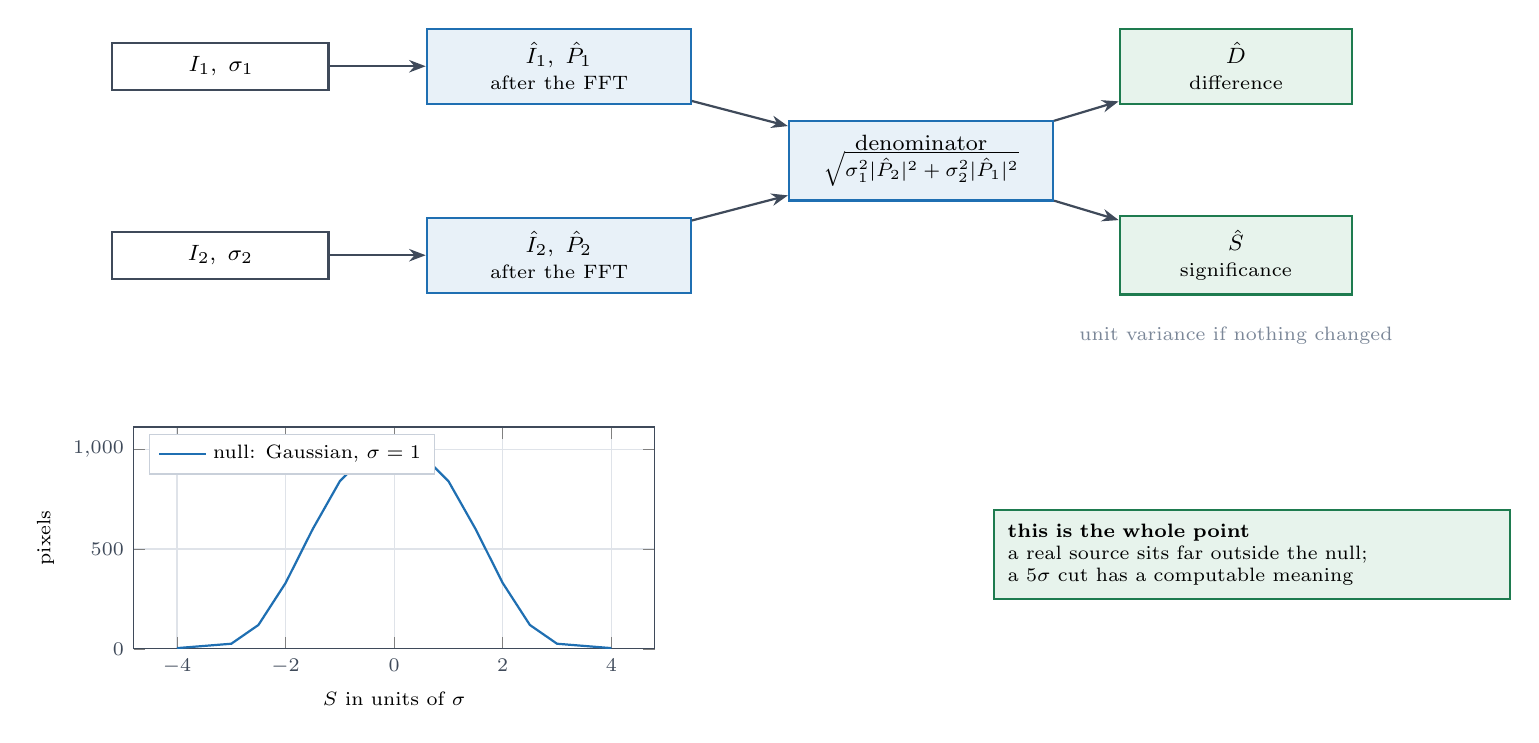
\begin{tikzpicture}[font=\footnotesize,
  v/.style={draw=slate,thick,fill=white,align=center,inner sep=5pt,text width=2.4cm},
  p/.style={draw=accent,thick,fill=accent2,align=center,inner sep=5pt,text width=3.0cm},
  o/.style={draw=good,thick,fill=good2,align=center,inner sep=5pt,text width=2.6cm},
  ar/.style={-{Stealth[length=6pt]},draw=slate,thick}]
  \node[v] (i1) at (1.5,4.2) {$I_1,\ \sigma_1$};
  \node[v] (i2) at (1.5,1.8) {$I_2,\ \sigma_2$};
  \node[p] (f1) at (5.8,4.2) {$\hat I_1,\ \hat P_1$\\ \scriptsize after the FFT};
  \node[p] (f2) at (5.8,1.8) {$\hat I_2,\ \hat P_2$\\ \scriptsize after the FFT};
  \node[p] (den) at (10.4,3.0) {denominator\\ \scriptsize $\sqrt{\sigma_1^2|\hat P_2|^2+\sigma_2^2|\hat P_1|^2}$};
  \node[o] (D) at (14.4,4.2) {$\hat D$\\ \scriptsize difference};
  \node[o] (S) at (14.4,1.8) {$\hat S$\\ \scriptsize significance};
  \draw[ar] (i1) -- (f1); \draw[ar] (i2) -- (f2);
  \draw[ar] (f1) -- (den); \draw[ar] (f2) -- (den);
  \draw[ar] (den) -- (D); \draw[ar] (den) -- (S);
  \node[below=4pt,text=muted,font=\scriptsize,align=center] at (14.4,1.15) {unit variance if nothing changed};
  % null histogram
  \begin{scope}[shift={(0.4,-3.2)}]
    \begin{axis}[width=8.2cm,height=4.4cm,
      xlabel={$S$ in units of $\sigma$},ylabel={pixels},
      xlabel style={font=\scriptsize},ylabel style={font=\scriptsize},
      tick label style={font=\scriptsize,text=slate},axis line style={slate},ymin=0,
      grid=major,grid style={rule!60},legend style={font=\scriptsize,draw=rule,at={(0.03,0.97)},anchor=north west}]
    \addplot[thick,accent,mark=none] coordinates {
      (-4,4) (-3,26) (-2.5,120) (-2,330) (-1.5,600) (-1,840) (-0.5,975) (0,1010)
      (0.5,975) (1,840) (1.5,600) (2,330) (2.5,120) (3,26) (4,4)};
    \addlegendentry{null: Gaussian, $\sigma=1$}
    \end{axis}
  \end{scope}
  \node[draw=good,thick,fill=good2,align=left,inner sep=5pt,text width=6.2cm,font=\scriptsize] at (14.6,-2.0)
    {\textbf{this is the whole point}\\ a real source sits far outside the null;\\ a $5\sigma$ cut has a computable meaning};
\end{tikzpicture}}

\textbf{Spoken script.} Stage three is the mathematical heart, and it is two lines. The classical approach
fits a kernel so that both images end up with the same PSF; ZOGY instead convolves both images to a common
PSF in Fourier space in a least-squares optimal way, and it never estimates a kernel from the data. Read
the first equation as a comparison: image two convolved with PSF one, image one convolved with PSF two,
and the difference normalised by exactly the noise that survives. The second equation turns that into a
significance, and here is the crucial property: where the sky did not change, S is Gaussian with zero
mean and unit variance. Not approximately -- by construction.\par
The histogram underneath is what that looks like: one clean peak at zero, one sigma wide, with any real
source far out in the tails. That is why a five-sigma threshold can be defended, and it is the entire
reason for choosing this algorithm over the simpler alternatives. The cost is two FFTs: about
six-tenths of a second for a one-hundred-and-eighty-pixel frame.

\newpage
% -------------------------------------------------------------- SLIDE 12 ---
\slidehead{12}{Theory III: what a threshold actually buys}{0:55}

\textbf{On the slide.}
\begin{itemize}[leftmargin=1.4em,itemsep=2pt,topsep=2pt]
\item If the null map is unit-variance, false positives are pure Gaussian tail:
      $\mathbb{E}[N_{\mathrm{FP}}]=N^2\Phi(-\tau)$
\item For $180^2=32\,400$ pixels: $3\sigma\Rightarrow219$, $4\sigma\Rightarrow11$, $5\sigma\Rightarrow0.018$
\item That is why the working threshold is five sigma and not three
\item Sanity check: measured detections are tens of sigma above this floor
\end{itemize}

\textbf{Figure / diagram.} The expected number of false pixels per frame against threshold, on a log
scale, with the three operating points marked and the working threshold drawn as a vertical line.

\figbox{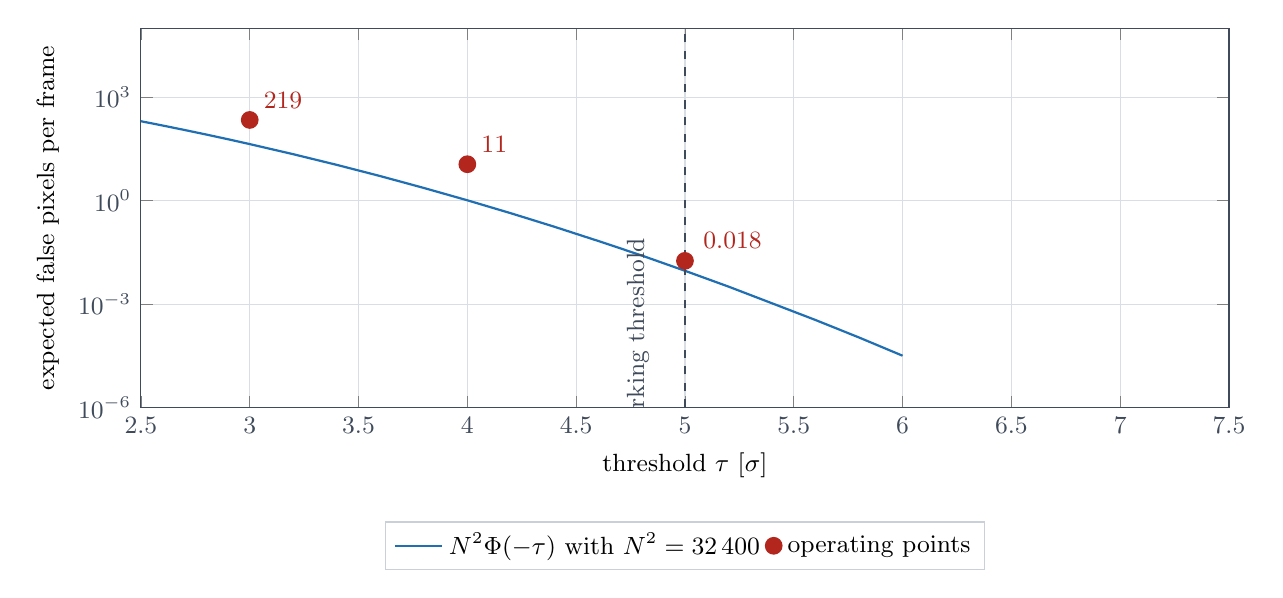
\begin{tikzpicture}[font=\footnotesize]
\begin{axis}[width=15.4cm,height=6.4cm,
  xlabel={threshold $\tau$ [$\sigma$]},ylabel={expected false pixels per frame},
  xlabel style={font=\small},ylabel style={font=\small},
  ymode=log,xmin=2.5,xmax=7.5,ymin=1e-6,ymax=1e5,
  grid=both,grid style={rule!70},axis line style={slate},
  tick label style={font=\small,text=slate},
  legend style={font=\small,draw=rule,at={(0.5,-0.30)},anchor=north,legend columns=2}]
\addplot[thick,accent,mark=none] coordinates {
  (2.5,201.2) (2.6,151.0) (2.7,112.3) (2.8,82.8) (2.9,60.5) (3.0,43.7)
  (3.2,22.26) (3.4,10.92) (3.6,5.16) (3.8,2.34) (4.0,1.026) (4.2,0.4324)
  (4.4,0.1754) (4.6,0.0684) (4.8,0.0259) (5.0,0.00929) (5.2,0.00323)
  (5.4,0.00106) (5.6,0.000347) (5.8,0.000108) (6.0,0.0000320)};
\addlegendentry{$N^2\Phi(-\tau)$ with $N^2=32\,400$}
\addplot[only marks,mark=*,mark size=3.0pt,bad] coordinates {(3,219) (4,11.4) (5,0.018)};
\addlegendentry{operating points}
\draw[dashed,slate,thick] (axis cs:5,1e-6) -- (axis cs:5,1e5);
\node[font=\small,text=slate,anchor=south,rotate=90] at (axis cs:4.88,1e-4) {working threshold};
\node[font=\small,text=bad,anchor=south west] at (axis cs:3.02,240) {219};
\node[font=\small,text=bad,anchor=south west] at (axis cs:4.02,13) {11};
\node[font=\small,text=bad,anchor=south west] at (axis cs:5.04,0.021) {0.018};
\end{axis}
\end{tikzpicture}}

\textbf{Spoken script.} Because the null distribution is analytic, the false-positive budget can be
computed rather than guessed, and that is the difference between a threshold and a wish. The curve is the
expected number of false pixels per frame as a function of threshold. At three sigma it is two hundred
and nineteen, so a single frame would be dominated by noise peaks. At four sigma, eleven. At five sigma,
nought point nought one eight -- one false pixel every fifty frames. That number is why the working
threshold is five sigma, and it is also why three-sigma detections in the literature need an external
prior before anyone believes them.\par
The sanity check runs the other way: the detection counts are far above this noise floor, tens of sigma
in several fields, so what is being looked at is structure rather than noise. That does not make the
detections real -- it only rules out the least interesting failure mode.

\newpage

% -------------------------------------------------------------- SLIDE 13 ---
\slidehead{13}{Theory IV: a dipole is a proper motion}{0:50}

\textbf{On the slide.}
\begin{itemize}[leftmargin=1.4em,itemsep=2pt,topsep=2pt]
\item A positive peak with a negative partner means the source moved: a dipole
\item A lone positive peak means it brightened: a monopole, that is variability
\item $\mu=s\,\Delta_{\mathrm{px}}/\Delta t$, valid for $0.5<\Delta_{\mathrm{px}}<25$\,px
\item Flux consistency $\eta=|S_++S_-|/|S_+-S_-|$ separates ``pure move'' from ``move and flare''
\end{itemize}

\textbf{Figure / diagram.} The geometry of a dipole with its separation vector and the conversion to
arcsec per year, beside the monopole case, and one worked example underneath.

\figbox{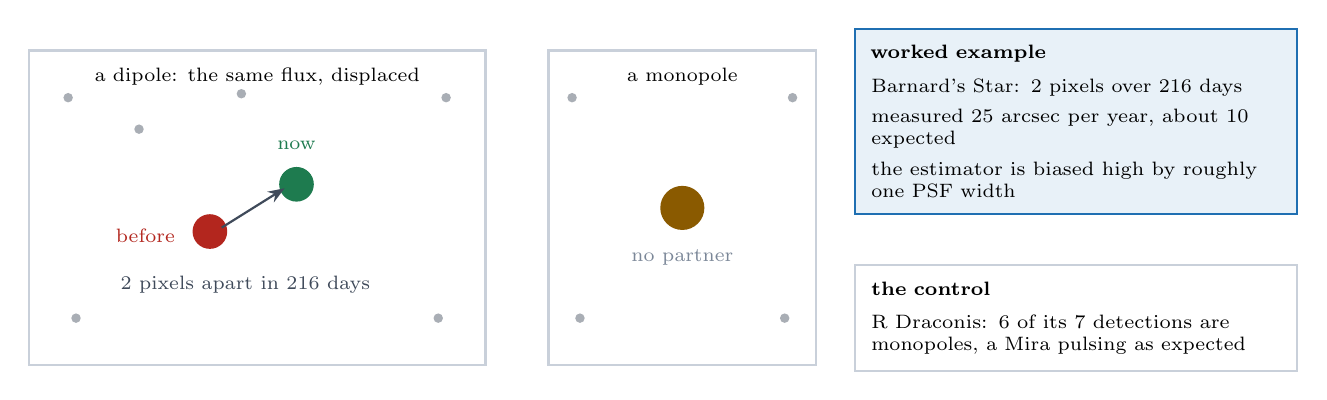
\begin{tikzpicture}[font=\footnotesize]
  \draw[rule,thick,fill=white] (0.3,2.6) rectangle (6.1,6.6);
  \node[anchor=north,font=\scriptsize] at (3.2,6.5) {a dipole: the same flux, displaced};
  \foreach \x/\y in {0.8/6.0,5.6/6.0,0.9/3.2,5.5/3.2,3.0/6.05,1.7/5.6}{\fill[slate!45] (\x,\y) circle (0.06);}
  \fill[bad] (2.6,4.3) circle (0.22);
  \fill[good] (3.7,4.9) circle (0.22);
  \draw[-{Stealth[length=6pt]},thick,slate] (2.75,4.35) -- (3.55,4.85);
  \node[anchor=north,font=\scriptsize,text=slate] at (3.05,3.86) {2 pixels apart in 216 days};
  \node[anchor=east,font=\scriptsize,text=bad] at (2.28,4.25) {before};
  \node[anchor=south,font=\scriptsize,text=good] at (3.70,5.22) {now};
  \draw[rule,thick,fill=white] (6.9,2.6) rectangle (10.3,6.6);
  \node[anchor=north,font=\scriptsize] at (8.6,6.5) {a monopole};
  \foreach \x/\y in {7.2/6.0,10.0/6.0,7.3/3.2,9.9/3.2}{\fill[slate!45] (\x,\y) circle (0.06);}
  \fill[warn] (8.6,4.6) circle (0.28);
  \node[anchor=north,font=\scriptsize,text=muted] at (8.6,4.2) {no partner};
  \node[draw=accent,thick,fill=accent2,align=left,inner sep=6pt,text width=5.2cm,font=\scriptsize] at (13.6,5.7)
    {\textbf{worked example}\\[4pt] Barnard's Star: 2 pixels over 216 days\\[3pt] measured 25 arcsec per year, about 10 expected\\[3pt] the estimator is biased high by roughly one PSF width};
  \node[draw=rule,thick,fill=white,align=left,inner sep=6pt,text width=5.2cm,font=\scriptsize] at (13.6,3.2)
    {\textbf{the control}\\[4pt] R Draconis: 6 of its 7 detections are monopoles, a Mira pulsing as expected};
\end{tikzpicture}}

\textbf{Spoken script.} Once there is a significance map, the morphology does the classifying, and it is
almost embarrassingly simple. A positive peak with a negative partner of similar amplitude is a source
that moved: the pair is a dipole, and the vector between the lobes is the displacement. Divide by the
time baseline and you have a proper motion. A positive peak with no partner is a source that brightened,
which is variability. Two guard rails: the separation must exceed half a pixel or you are pairing
PSF-correlated noise, and stay below twenty-five pixels or you are pairing with an unrelated trough
across the frame. There is also a flux-consistency statistic -- how asymmetric the two lobes are -- which
separates a rigid displacement from an object that moved and changed brightness at once.\par
Barnard's Star is the worked example: two pixels in two hundred and sixteen days. The measured proper
motion comes out at about twenty-five arcseconds a year against a true value of ten, and the reason is on
the slide -- peak separations are biased high by roughly one PSF width. R Draconis is the control: six
of its seven detections are monopoles, which is what a pulsating Mira should give.

\newpage
% -------------------------------------------------------------- SLIDE 14 ---
\slidehead{14}{Theory V: triage is a second hypothesis test}{0:55}

\textbf{On the slide.}
\begin{itemize}[leftmargin=1.4em,itemsep=2pt,topsep=2pt]
\item Pixel to sky with the flat approximation: $\alpha=\alpha_0-(x-N/2)s/3600$
\item Nearest neighbour in Gaia DR3, AllWISE and VSX; verdict at $30\arcsec$, confidence at $5\arcsec$
\item Loose on purpose: the PSF is $4\arcsec$, and a tight radius inflates the candidate list
\item The trap: position-only matching fails for fast movers, because the epochs differ
\end{itemize}

\textbf{Figure / diagram.} The two match radii around a detection on the left, the verdict flow on the
right, and underneath the failure mode that this radius creates for a high-proper-motion star.

\figbox{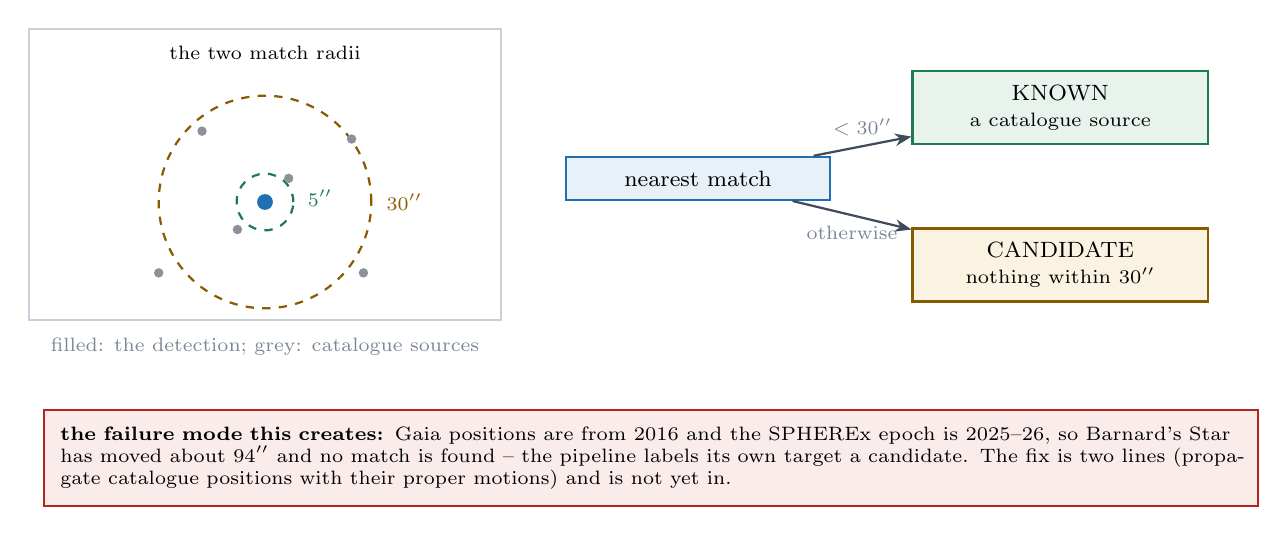
\begin{tikzpicture}[font=\footnotesize,
  k/.style={draw=good,thick,fill=good2,align=center,inner sep=5pt,text width=3.4cm},
  c/.style={draw=warn,thick,fill=warn2,align=center,inner sep=5pt,text width=3.4cm},
  m/.style={draw=accent,thick,fill=accent2,align=center,inner sep=5pt,text width=3.0cm},
  ar/.style={-{Stealth[length=6pt]},draw=slate,thick}]
  \draw[rule,thick,fill=white] (0.3,2.9) rectangle (6.3,6.6);
  \node[anchor=north,font=\scriptsize] at (3.3,6.5) {the two match radii};
  \draw[warn,dashed,thick] (3.3,4.4) circle (1.35);
  \draw[good,dashed,thick] (3.3,4.4) circle (0.36);
  \fill[accent] (3.3,4.4) circle (0.10);
  \foreach \x/\y in {3.6/4.7,2.95/4.05,4.4/5.2,1.95/3.5,2.5/5.3,4.55/3.5}{\fill[slate!60] (\x,\y) circle (0.06);}
  \node[anchor=west,font=\scriptsize,text=good] at (3.72,4.45) {5\arcsec};
  \node[anchor=west,font=\scriptsize,text=warn] at (4.72,4.40) {30\arcsec};
  \node[anchor=north,font=\scriptsize,text=muted] at (3.3,2.8) {filled: the detection; grey: catalogue sources};
  \node[m] (mt) at (8.8,4.7) {nearest match};
  \node[k] (kn) at (13.4,5.6) {KNOWN\\ \scriptsize a catalogue source};
  \node[c] (ca) at (13.4,3.6) {CANDIDATE\\ \scriptsize nothing within $30\arcsec$};
  \draw[ar] (mt) -- node[above,font=\scriptsize,text=muted] {$<30\arcsec$} (kn);
  \draw[ar] (mt) -- node[below,font=\scriptsize,text=muted] {otherwise} (ca);
  \node[draw=bad,thick,fill=bad2,align=left,inner sep=6pt,text width=15.0cm,font=\scriptsize] at (8.2,1.15)
    {\textbf{the failure mode this creates:} Gaia positions are from 2016 and the SPHEREx epoch is 2025--26, so Barnard's Star has moved about 94\arcsec{} and no match is found -- the pipeline labels its own target a candidate. The fix is two lines (propagate catalogue positions with their proper motions) and is not yet in.};
\end{tikzpicture}}

\textbf{Spoken script.} A detection is not a discovery until you have asked whether something was already
there, and that is a second hypothesis test: is the nearest catalogue source consistent with this
position? The pixel is converted to sky with a flat approximation -- legitimate at nine arcminutes -- and
the nearest source is looked up in Gaia, WISE and the variable-star index. Thirty arcseconds is the
verdict radius, five arcseconds grades the confidence.\par
Both numbers are deliberately loose and I want to defend that: the PSF is four arcseconds across, so a
tight radius would miss real counterparts and flatter me with false candidates. The red box is what that
choice costs. Gaia measured positions in 2016, these images are from 2025, and Barnard's Star -- the
fastest star in the sky -- has moved ninety-four arcseconds in between, far outside any match radius. So
the pipeline labels my own target as an unexplained candidate. The fix is standard practice: propagate
the catalogue positions to the epoch of observation with their proper motions. It is a two-line change,
and it is not yet in, which is exactly why slide twenty-two says seventeen candidates and not five.

\newpage

% -------------------------------------------------------------- SLIDE 15 ---
\slidehead{15}{Theory VI: a spectrum per detection, for free}{0:45}

\textbf{On the slide.}
\begin{itemize}[leftmargin=1.4em,itemsep=2pt,topsep=2pt]
\item Every pixel knows its wavelength, so aperture photometry per band gives a low-resolution spectrum
\item Three indices: CH$_4$ at 1.6/1.74, H$_2$O continuum over troughs, NIR slope 4.6/1.1
\item T dwarf: strong methane; L dwarf: water; a hot star or quasar: a red power law
\item The classifier reports the three indices, never a bare label
\end{itemize}

\textbf{Figure / diagram.} The wavelength axis with the index band-pairs shaded, and three schematic
spectra underneath showing what each index is for.

\figbox{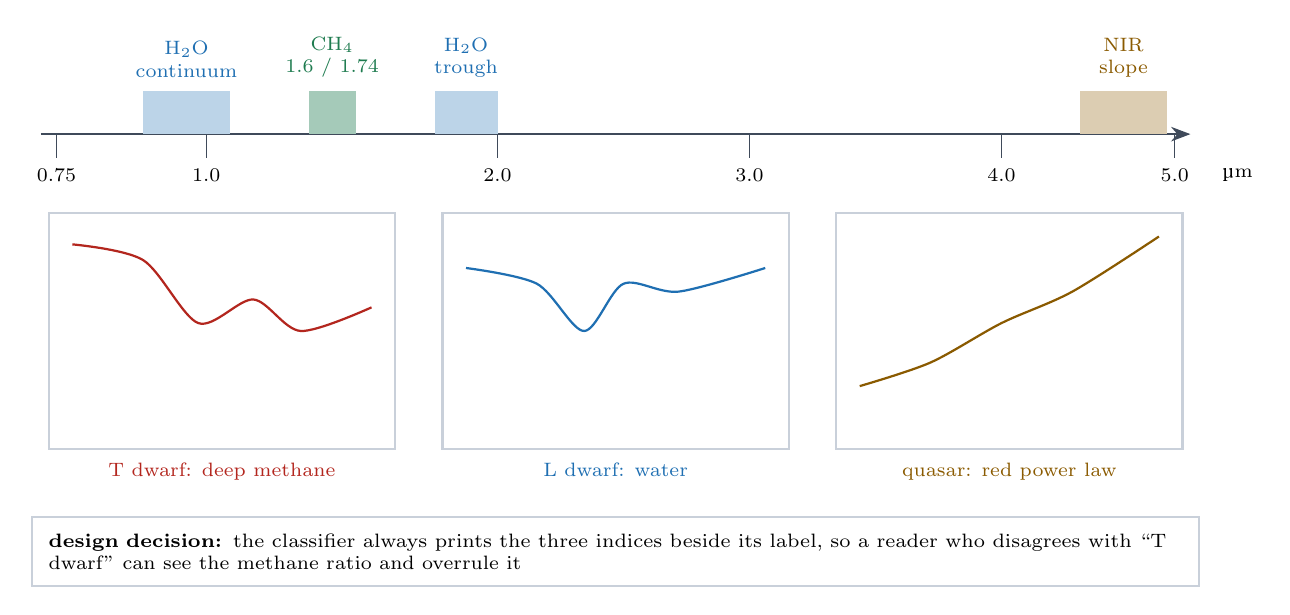
\begin{tikzpicture}[font=\footnotesize]
  \draw[-{Stealth[length=7pt]},thick,slate] (0.2,5.6) -- (14.8,5.6);
  \foreach \w/\x in {0.75/0.4,1.0/2.3,2.0/6.0,3.0/9.2,4.0/12.4,5.0/14.6}{\draw[slate] (\x,5.6) -- (\x,5.3); \node[anchor=north,font=\scriptsize] at (\x,5.28) {\w};}
  \node[anchor=north,font=\scriptsize] at (15.4,5.28) {\textmu m};
  \fill[accent!30] (1.5,5.6) rectangle (2.6,6.15);
  \node[anchor=south,font=\scriptsize,align=center,text=accent] at (2.05,6.2) {H$_2$O\\ continuum};
  \fill[good!40] (3.6,5.6) rectangle (4.2,6.15);
  \node[anchor=south,font=\scriptsize,align=center,text=good] at (3.9,6.2) {CH$_4$\\ 1.6 / 1.74};
  \fill[accent!30] (5.2,5.6) rectangle (6.0,6.15);
  \node[anchor=south,font=\scriptsize,align=center,text=accent] at (5.6,6.2) {H$_2$O\\ trough};
  \fill[warn!30] (13.4,5.6) rectangle (14.5,6.15);
  \node[anchor=south,font=\scriptsize,align=center,text=warn] at (13.95,6.2) {NIR\\ slope};
  % three schematic spectra
  \draw[rule,thick,fill=white] (0.3,1.6) rectangle (4.7,4.6);
  \draw[bad,thick] plot[smooth] coordinates {(0.6,4.2) (1.5,4.0) (2.2,3.2) (2.9,3.5) (3.5,3.1) (4.4,3.4)};
  \node[anchor=north,font=\scriptsize,text=bad] at (2.5,1.55) {T dwarf: deep methane};
  \draw[rule,thick,fill=white] (5.3,1.6) rectangle (9.7,4.6);
  \draw[accent,thick] plot[smooth] coordinates {(5.6,3.9) (6.5,3.7) (7.1,3.1) (7.6,3.7) (8.3,3.6) (9.4,3.9)};
  \node[anchor=north,font=\scriptsize,text=accent] at (7.5,1.55) {L dwarf: water};
  \draw[rule,thick,fill=white] (10.3,1.6) rectangle (14.7,4.6);
  \draw[warn,thick] plot[smooth] coordinates {(10.6,2.4) (11.5,2.7) (12.4,3.2) (13.3,3.6) (14.4,4.3)};
  \node[anchor=north,font=\scriptsize,text=warn] at (12.5,1.55) {quasar: red power law};
  \node[draw=rule,thick,fill=white,align=left,inner sep=6pt,text width=14.4cm,font=\scriptsize] at (7.5,0.3)
    {\textbf{design decision:} the classifier always prints the three indices beside its label, so a reader who disagrees with ``T dwarf'' can see the methane ratio and overrule it};
\end{tikzpicture}}

\textbf{Spoken script.} The last piece of theory is nearly free, and it is why SPHEREx is interesting for
this kind of work. Because every pixel carries its wavelength in a table, measuring an aperture in each
band gives a low-resolution spectrum of the detection without any follow-up telescope. It reduces to
three numbers that are physically motivated: methane absorption at one-point-six over one-point-seven-four
microns marks a T dwarf; water, the ratio of continuum to trough, marks an L dwarf; and the slope from
one to four-point-six microns separates stars from a red power law, which is a dusty galaxy or a quasar.\par
The three little spectra underneath are what those cases look like. The important design decision is in
the bottom box: the classifier prints the three indices next to its label, never the label alone, so a
reader who disagrees can see the methane ratio and overrule it.

\newpage
% -------------------------------------------------------------- SLIDE 16 ---
\slidehead{16}{Validation: injection and recovery}{0:55}

\textbf{On the slide.}
\begin{itemize}[leftmargin=1.4em,itemsep=2pt,topsep=2pt]
\item Synthetic sources are planted at known SNR and proper motion, then stages two and three re-run
\item A trial counts as recovered if a detection of the right class lands within 2\,px
\item The output is a $6\times4$ matrix, never a single number: the proper-motion axis is the point
\item Result on real frames: near-zero. The test is measuring the wrong amplitude
\end{itemize}

\textbf{Figure / diagram.} Left: the measured recovery matrix as a heat map. Right: why it fails -- the
variance plane the injection uses against the residual structure the data actually contain.

\figbox{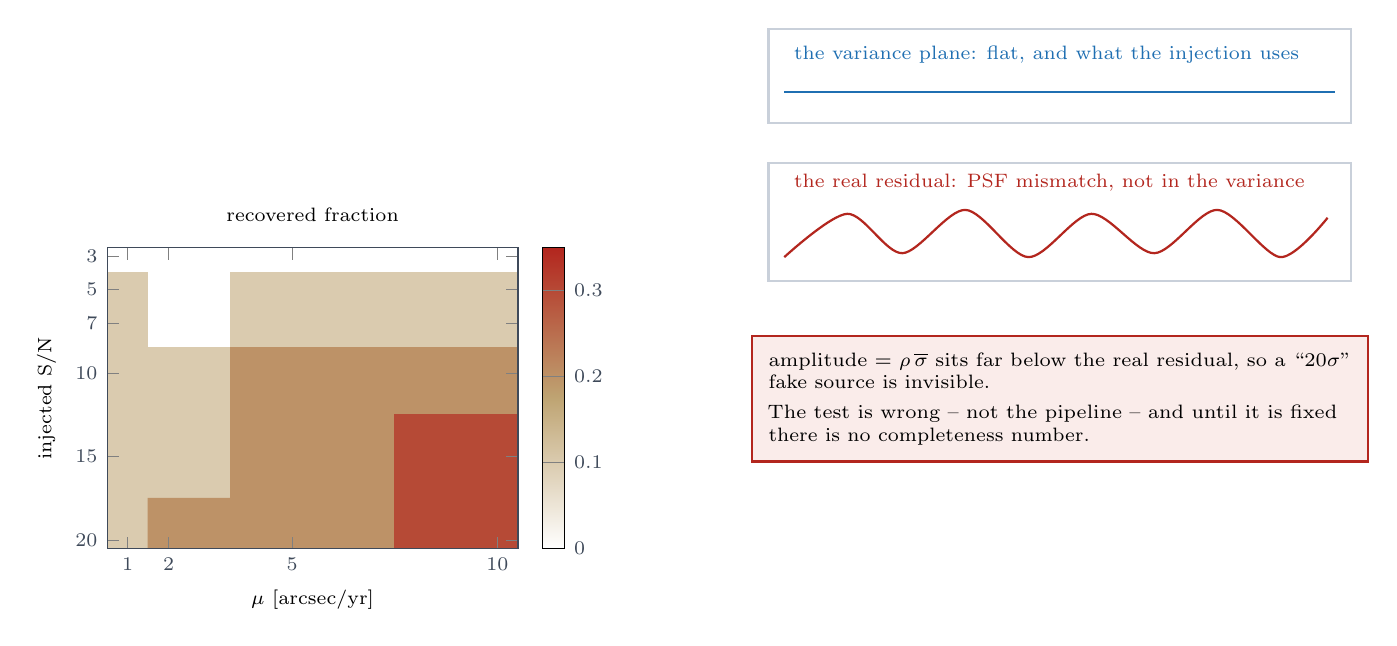
\begin{tikzpicture}[font=\footnotesize]
  \begin{scope}
    \begin{axis}[width=6.8cm,height=5.4cm,
      view={0}{90},colormap={rec}{color=(white) color=(warn!55) color=(bad)},
      colorbar,colorbar style={font=\scriptsize,width=0.28cm},
      xlabel={$\mu$ [arcsec/yr]},ylabel={injected S/N},
      xlabel style={font=\scriptsize},ylabel style={font=\scriptsize},
      xtick={1,2,5,10},ytick={3,5,7,10,15,20},xmin=0.5,xmax=10.5,ymin=2.5,ymax=20.5,
      tick label style={font=\scriptsize,text=slate},axis line style={slate},
      point meta min=0,point meta max=0.35,
      title={recovered fraction},title style={font=\scriptsize}]
    \addplot[matrix plot,mesh/cols=4,mesh/rows=6,point meta=explicit] coordinates {
      (1,3)[0.0] (2,3)[0.0] (5,3)[0.0] (10,3)[0.0]
      (1,5)[0.1] (2,5)[0.0] (5,5)[0.1] (10,5)[0.1]
      (1,7)[0.1] (2,7)[0.0] (5,7)[0.1] (10,7)[0.1]
      (1,10)[0.1] (2,10)[0.1] (5,10)[0.2] (10,10)[0.2]
      (1,15)[0.1] (2,15)[0.1] (5,15)[0.2] (10,15)[0.3]
      (1,20)[0.1] (2,20)[0.2] (5,20)[0.2] (10,20)[0.3]};
    \end{axis}
  \end{scope}
  \draw[rule,thick,fill=white] (8.4,5.4) rectangle (15.8,6.6);
  \draw[accent,thick] (8.6,5.8) -- (15.6,5.8);
  \node[anchor=north west,font=\scriptsize,text=accent] at (8.6,6.5) {the variance plane: flat, and what the injection uses};
  \draw[rule,thick,fill=white] (8.4,3.4) rectangle (15.8,4.9);
  \draw[bad,thick] plot[smooth] coordinates {(8.6,3.70) (9.4,4.25) (10.1,3.75) (10.9,4.30) (11.7,3.70) (12.5,4.25) (13.3,3.75) (14.1,4.30) (14.9,3.70) (15.5,4.20)};
  \node[anchor=north west,font=\scriptsize,text=bad] at (8.6,4.88) {the real residual: PSF mismatch, not in the variance};
  \node[draw=bad,thick,fill=bad2,align=left,inner sep=6pt,text width=7.4cm,font=\scriptsize] at (12.1,1.9)
    {amplitude $=\rho\,\overline{\sigma}$ sits far below the real residual, so a ``20$\sigma$'' fake source is invisible.\\[3pt] The test is wrong -- not the pipeline -- and until it is fixed there is no completeness number.};
\end{tikzpicture}}

\textbf{Spoken script.} A detection chain is only as good as its completeness curve, so stage six plants
fake sources and counts how many come back. The grid is signal-to-noise from three to twenty, proper
motion from one to ten arcseconds per year, twenty trials per cell, and a trial counts if the right kind
of detection lands within two pixels of the injection.\par
And here is the uncomfortable result, which I am showing rather than hiding. On real frames almost
nothing is recovered: for Barnard's Star, zero out of twenty-four cells; the best field reaches three in
ten only at the brightest end. The reason is on the right. The amplitude that gets injected is tied to
the mean of the variance plane, which is flat, while the real residual in a co-added frame is dominated
by PSF mismatch, which is not in the variance plane at all. So a fake source injected at ``twenty sigma''
is a barely visible bump on top of the real residual. The test measures the wrong thing, and until that
is fixed there is no completeness limit -- which is why the results slides say unexplained rather than
new.

\newpage
% -------------------------------------------------------------- SLIDE 17 ---
\slidehead{17}{Implementation I: the code, and what changed}{1:05}

\textbf{On the slide.}
\begin{itemize}[leftmargin=1.4em,itemsep=2pt,topsep=2pt]
\item Six stage scripts (1\,318 lines), the service (808), the front end (1\,586): 6\,154 in total
\item Every stage is importable and runnable on its own, including on synthetic data
\item Five revisions turned a demo into a system, and each one was a bug with a lesson
\item Everything is deterministic; one metadata file is the contract between stages
\end{itemize}

\textbf{Figure / diagram.} Lines of code per module on the left, and on the right the revision that
matters most -- the guard that stops the service printing a meaningless noise estimate.

\figbox{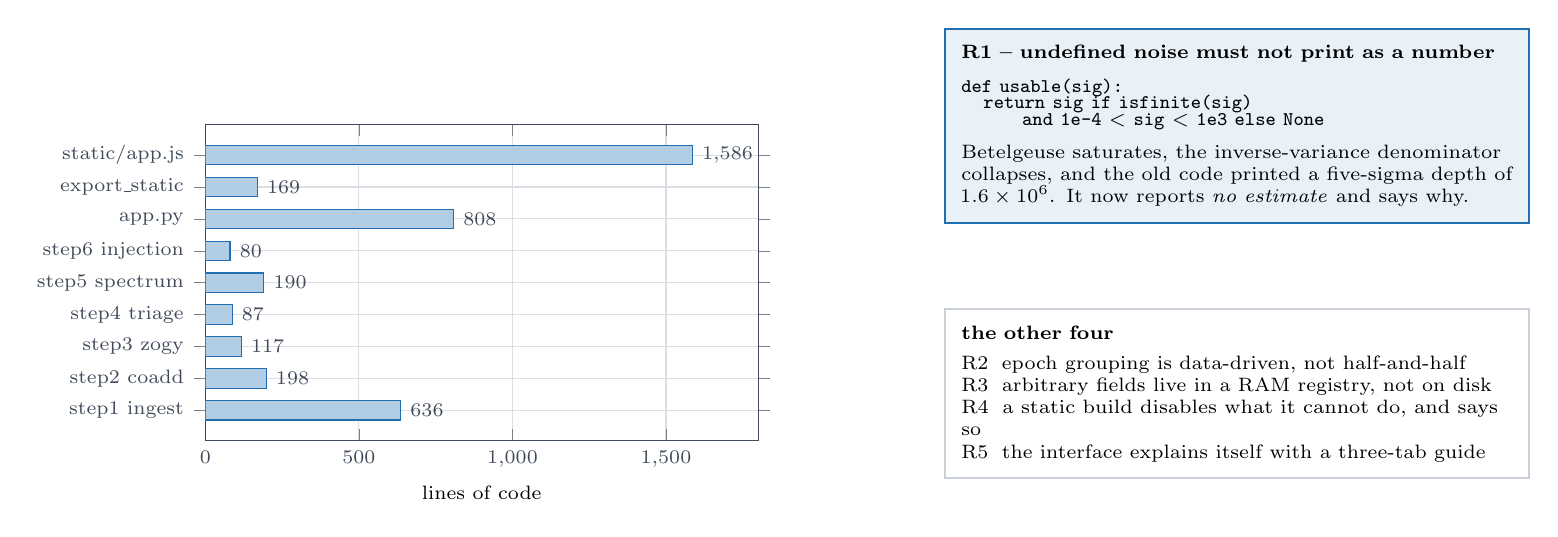
\begin{tikzpicture}[font=\footnotesize]
  \begin{scope}
    \begin{axis}[width=8.6cm,height=5.6cm,xbar,bar width=7pt,xmin=0,xmax=1800,
      xlabel={lines of code},xlabel style={font=\scriptsize},
      symbolic y coords={{step1 ingest},{step2 coadd},{step3 zogy},{step4 triage},{step5 spectrum},{step6 injection},{app.py},{export\_static},{static/app.js}},
      ytick=data,tick label style={font=\scriptsize,text=slate},axis line style={slate},
      grid=major,grid style={rule!70},nodes near coords,nodes near coords style={font=\scriptsize,text=slate},
      enlarge y limits=0.12]
    \addplot[fill=accent!35,draw=accent] coordinates {
      (636,{step1 ingest}) (198,{step2 coadd}) (117,{step3 zogy}) (87,{step4 triage})
      (190,{step5 spectrum}) (80,{step6 injection}) (808,{app.py}) (169,{export\_static})
      (1586,{static/app.js})};
    \end{axis}
  \end{scope}
  \begin{scope}[shift={(9.6,0.4)}]
    \node[draw=accent,thick,fill=accent2,align=left,inner sep=6pt,text width=7.0cm,font=\scriptsize] at (3.5,3.6)
      {\textbf{R1 -- undefined noise must not print as a number}\\[4pt]
       {\ttfamily def usable(sig):}\\[-2pt]
       {\ttfamily\hspace*{8pt}return sig if isfinite(sig)}\\[-2pt]
       {\ttfamily\hspace*{8pt}\hspace*{14pt}and 1e-4 $<$ sig $<$ 1e3 else None}\\[4pt]
       Betelgeuse saturates, the inverse-variance denominator collapses, and the old code printed a five-sigma depth of $1.6\times10^{6}$. It now reports \emph{no estimate} and says why.};
    \node[draw=rule,thick,fill=white,align=left,inner sep=6pt,text width=7.0cm,font=\scriptsize] at (3.5,0.2)
      {\textbf{the other four}\\[3pt]
       R2\; epoch grouping is data-driven, not half-and-half\\
       R3\; arbitrary fields live in a RAM registry, not on disk\\
       R4\; a static build disables what it cannot do, and says so\\
       R5\; the interface explains itself with a three-tab guide};
  \end{scope}
\end{tikzpicture}}

\textbf{Spoken script.} On the engineering. The pipeline is six scripts totalling about thirteen hundred
lines, one service of eight hundred, and a front end of sixteen hundred -- six thousand one hundred and
fifty-four in total, small enough that a reviewer can read all of it in an afternoon. Each stage has its
own entry point, so a single stage can be re-run on cached data when something looks wrong.\par
Five revisions matter enough to name. The most instructive is R1, on the right: Betelgeuse saturates the
detector, almost every pixel is flagged, the inverse-variance denominator collapses, and the old code
happily reported a five-sigma depth of one point six million. That is worse than reporting nothing,
because it looks like a measurement. The fix is four lines: anything outside a physically possible range
becomes ``no estimate'', with a note explaining why. The other four are the same flavour of honesty --
data-driven epoch grouping, a RAM registry for arbitrary fields, a static build that disables what it
cannot do, and an interface that explains itself.

\newpage

% -------------------------------------------------------------- SLIDE 18 ---
\slidehead{18}{Implementation II: one result set, three deployments}{0:55}

\textbf{On the slide.}
\begin{itemize}[leftmargin=1.4em,itemsep=2pt,topsep=2pt]
\item Live: FastAPI, five read-only endpoints, a 30-minute in-RAM cache, nothing written
\item Static: every response pre-rendered to JSON -- 28\,MB, and it works with no server at all
\item Hybrid: a static page plus a same-origin proxy, discovered by one probe at load
\item A static build disables ``live from IRSA'' and says why, instead of failing silently
\end{itemize}

\textbf{Figure / diagram.} The three shapes in three columns, with the request path drawn for each and
the latency written underneath.

\figbox{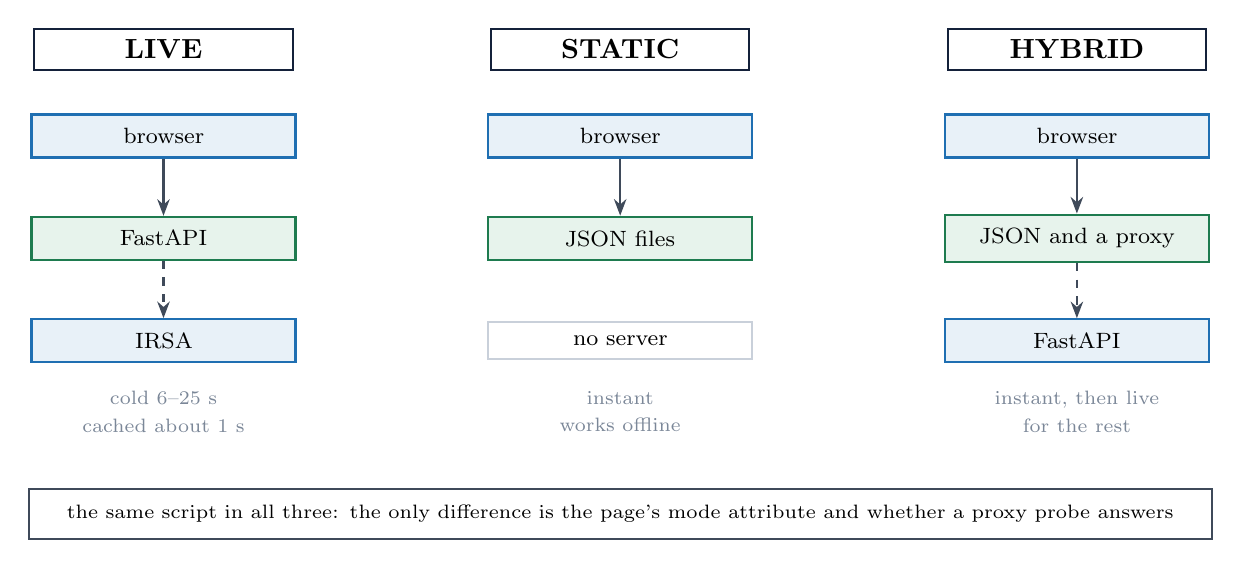
\begin{tikzpicture}[font=\footnotesize,
  hd/.style={draw=ink,thick,fill=white,align=center,inner sep=4pt,text width=3.0cm,font=\bfseries},
  bx/.style={draw=accent,thick,fill=accent2,align=center,inner sep=5pt,text width=3.0cm},
  st/.style={draw=good,thick,fill=good2,align=center,inner sep=5pt,text width=3.0cm},
  ar/.style={-{Stealth[length=6pt]},draw=slate,thick}]
  \node[hd] at (2.2,6.6) {LIVE};
  \node[hd] at (8.0,6.6) {STATIC};
  \node[hd] at (13.8,6.6) {HYBRID};
  \node[bx] (b1) at (2.2,5.5) {browser};
  \node[st] (a1) at (2.2,4.2) {FastAPI};
  \node[bx] (i1) at (2.2,2.9) {IRSA};
  \draw[ar] (b1) -- (a1); \draw[ar,dashed] (a1) -- (i1);
  \node[font=\scriptsize,text=muted,align=center] at (2.2,2.0) {cold 6--25 s\\[2pt] cached about 1 s};
  \node[bx] (b2) at (8.0,5.5) {browser};
  \node[st] (a2) at (8.0,4.2) {JSON files};
  \node[draw=rule,thick,fill=white,align=center,inner sep=5pt,text width=3.0cm] (i2) at (8.0,2.9) {no server};
  \draw[ar] (b2) -- (a2);
  \node[font=\scriptsize,text=muted,align=center] at (8.0,2.0) {instant\\[2pt] works offline};
  \node[bx] (b3) at (13.8,5.5) {browser};
  \node[st] (a3) at (13.8,4.2) {JSON and a proxy};
  \node[bx] (i3) at (13.8,2.9) {FastAPI};
  \draw[ar] (b3) -- (a3); \draw[ar,dashed] (a3) -- (i3);
  \node[font=\scriptsize,text=muted,align=center] at (13.8,2.0) {instant, then live\\[2pt] for the rest};
  \node[draw=slate,thick,fill=white,align=center,inner sep=6pt,text width=14.6cm,font=\scriptsize] at (8.0,0.7)
    {the same script in all three: the only difference is the page's mode attribute and whether a proxy probe answers};
\end{tikzpicture}}

\textbf{Spoken script.} The last piece of engineering is how the result is served, and it is deliberately
built in three shapes because each answers a different question. Live: a service with five read-only
endpoints, a thirty-minute in-RAM cache and nothing written to disk -- thirty to sixty seconds for a cold
field, about a second when cached. Static: a script renders every response for every field to JSON, which
is twenty-eight megabytes and works from a USB stick with no server. Hybrid: a static page with a
same-origin proxy to a Python host, which is how a static host can still offer the live features.\par
One consequence is a principle rather than a detail. On the pure static deployment, live fetching cannot
work -- so the page disables that control, relabels it ``live from IRSA, needs a backend'', and prints the
reason underneath. If a proxy appears later, a single probe turns it back on. A toggle that silently does
nothing is worse than one that is switched off.

\newpage
% -------------------------------------------------------------- SLIDE 19 ---
\slidehead{19}{Implementation III: the front end}{0:45}

\textbf{On the slide.}
\begin{itemize}[leftmargin=1.4em,itemsep=2pt,topsep=2pt]
\item 1\,586 lines of plain JavaScript: no framework, no build step, no tracker
\item A canvas engine with three layers (co-add, difference, significance) plus overlays
\item One JSON per field carries the map, the detections, the objects, the spectrum and the provenance
\item A three-tab guide written for someone who has never seen an astronomical image
\end{itemize}

\textbf{Figure / diagram.} A wireframe of the actual page with the panels labelled, and the three-layer
canvas stack drawn beside it.

\figbox{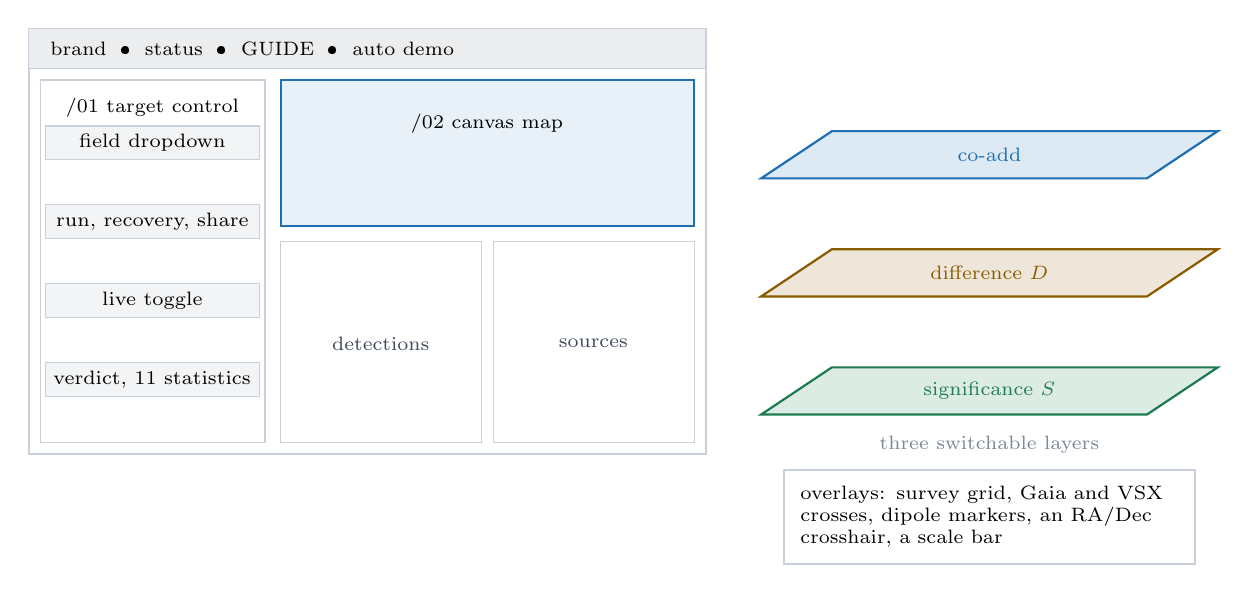
\begin{tikzpicture}[font=\footnotesize]
  % wireframe
  \draw[rule,thick,fill=white] (0.3,1.4) rectangle (8.9,6.8);
  \draw[rule,fill=slate!10] (0.3,6.3) rectangle (8.9,6.8);
  \node[anchor=west,font=\scriptsize] at (0.45,6.55) {brand \;\textbullet\; status \;\textbullet\; GUIDE \;\textbullet\; auto demo};
  \draw[rule,fill=white] (0.45,1.55) rectangle (3.30,6.15);
  \node[anchor=north,font=\scriptsize] at (1.87,6.05) {/01 target control};
  \node[draw=rule,fill=slate!6,align=center,inner sep=3pt,text width=2.5cm,font=\scriptsize] at (1.87,5.35) {field dropdown};
  \node[draw=rule,fill=slate!6,align=center,inner sep=3pt,text width=2.5cm,font=\scriptsize] at (1.87,4.35) {run, recovery, share};
  \node[draw=rule,fill=slate!6,align=center,inner sep=3pt,text width=2.5cm,font=\scriptsize] at (1.87,3.35) {live toggle};
  \node[draw=rule,fill=slate!6,align=center,inner sep=3pt,text width=2.5cm,font=\scriptsize] at (1.87,2.35) {verdict, 11 statistics};
  \draw[accent,thick,fill=accent2] (3.50,4.30) rectangle (8.75,6.15);
  \node[font=\scriptsize] at (6.12,5.6) {/02 canvas map};
  \draw[rule,fill=white] (3.50,1.55) rectangle (6.05,4.10);
  \node[font=\scriptsize,text=slate] at (4.77,2.8) {detections};
  \draw[rule,fill=white] (6.20,1.55) rectangle (8.75,4.10);
  \node[font=\scriptsize,text=slate] at (7.47,2.8) {sources};
  % layer stack with labels inside
  \foreach \i/\lab/\col in {0/{significance $S$}/good,1/{difference $D$}/warn,2/{co-add}/accent}{
    \draw[\col,thick,fill=\col!15] (9.6,\i*1.5+1.9) -- (10.5,\i*1.5+2.5) -- (15.4,\i*1.5+2.5) -- (14.5,\i*1.5+1.9) -- cycle;
    \node[font=\scriptsize,text=\col] at (12.5,\i*1.5+2.2) {\lab};}
  \node[anchor=north,font=\scriptsize,text=muted] at (12.5,1.75) {three switchable layers};
  \node[draw=rule,thick,fill=white,align=left,inner sep=6pt,text width=4.8cm,font=\scriptsize] at (12.5,0.6)
    {overlays: survey grid, Gaia and VSX crosses, dipole markers, an RA/Dec crosshair, a scale bar};
\end{tikzpicture}}

\textbf{Spoken script.} The front end is sixteen hundred lines of plain JavaScript, with no framework and
no build step, which is why it will still run in five years. It is a small canvas engine with three
switchable layers -- the co-add, the difference image and the significance map -- plus overlays for the
survey grid, the catalogue positions, the dipole markers and a readout of whatever is under the cursor.
On the left of the wireframe, target control: pick a field, run, read the verdict and eleven statistics,
or ask for a recovery grid.\par
The thing to point at is the Guide button in the top bar. It opens three tabs written for someone who has
never looked at an astronomical image: how it works, how to use this page click by click, and a glossary
of the ten words that matter. It is plain HTML inside the page, so it ships in the static build and needs
no backend -- and it states the backend limitation in the same place as everything else.

\newpage

% -------------------------------------------------------------- SLIDE 20 ---
\slidehead{20}{Results I: eighteen fields, eighty-eight detections}{1:05}

\textbf{On the slide.}
\begin{itemize}[leftmargin=1.4em,itemsep=2pt,topsep=2pt]
\item 88 detections over 18 fields: 71 KNOWN (81\%) and 17 CANDIDATE
\item Detection count is not discovery count: M1, Sirius and R Draconis are 100\% explained
\item The amber bars -- WISE 0855, Epsilon Indi B, Barnard's Star -- are the interesting ones
\item Four fields produce nothing usable, and they are on the next slide
\end{itemize}

\textbf{Figure / diagram.} Stacked bars for all eighteen fields, visually grouped into the five brief
targets and the thirteen famous objects, with the totals in the caption strip.

\figbox{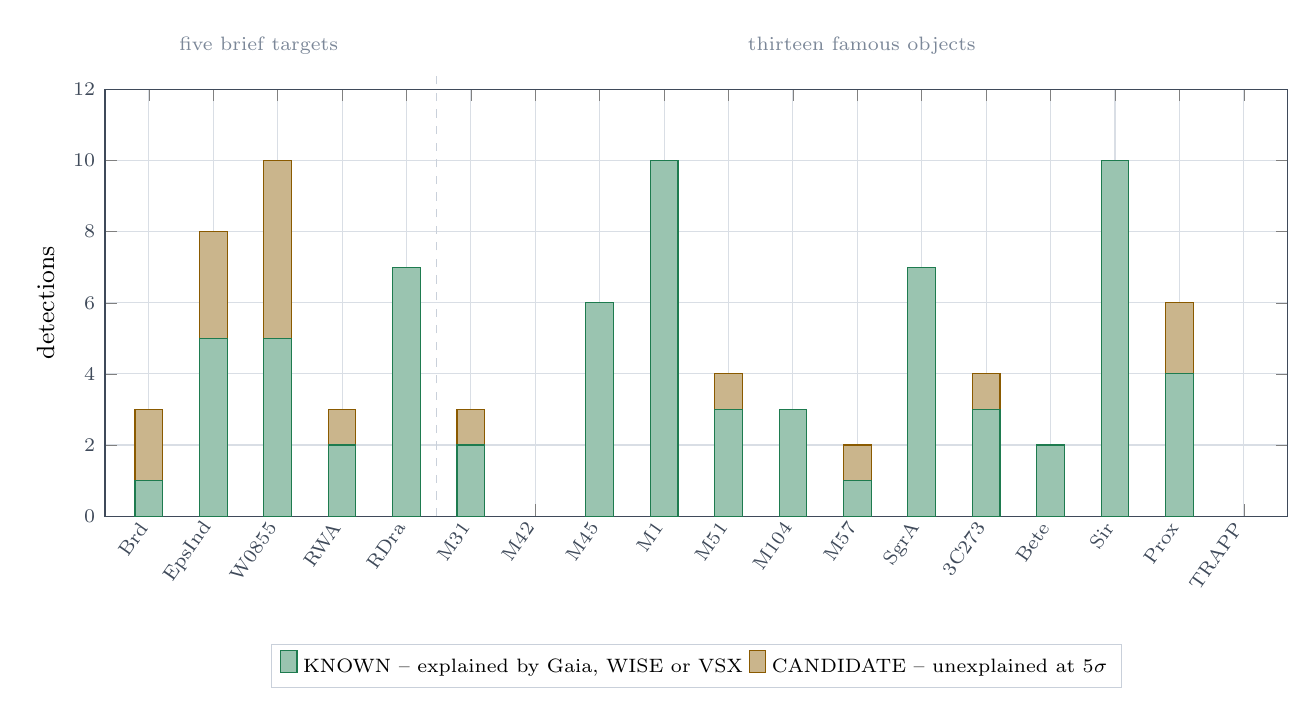
\begin{tikzpicture}[font=\footnotesize]
\begin{axis}[width=16.6cm,height=7.0cm,
  ybar stacked,bar width=10pt,ymin=0,ymax=12,ylabel={detections},
  ylabel style={font=\small},
  symbolic x coords={{Brd},{EpsInd},{W0855},{RWA},{RDra},{M31},{M42},{M45},{M1},{M51},{M104},{M57},{SgrA},{3C273},{Bete},{Sir},{Prox},{TRAPP}},
  xtick=data,x tick label style={rotate=55,anchor=east,font=\scriptsize},
  tick label style={font=\scriptsize,text=slate},axis line style={slate},
  grid=major,grid style={rule!70},enlarge x limits=0.04,
  legend style={font=\scriptsize,draw=rule,at={(0.5,-0.30)},anchor=north,legend columns=2},
  after end axis/.code={
    \draw[rule,dashed] (rel axis cs:0.28,0) -- (rel axis cs:0.28,1.05);
    \node[font=\scriptsize,text=muted,anchor=south] at (rel axis cs:0.13,1.06) {five brief targets};
    \node[font=\scriptsize,text=muted,anchor=south] at (rel axis cs:0.64,1.06) {thirteen famous objects};}]
\addplot[fill=good!45,draw=good] coordinates {
  ({Brd},1) ({EpsInd},5) ({W0855},5) ({RWA},2) ({RDra},7) ({M31},2) ({M42},0) ({M45},6) ({M1},10)
  ({M51},3) ({M104},3) ({M57},1) ({SgrA},7) ({3C273},3) ({Bete},2) ({Sir},10) ({Prox},4) ({TRAPP},0)};
\addlegendentry{KNOWN -- explained by Gaia, WISE or VSX}
\addplot[fill=warn!45,draw=warn] coordinates {
  ({Brd},2) ({EpsInd},3) ({W0855},5) ({RWA},1) ({RDra},0) ({M31},1) ({M42},0) ({M45},0) ({M1},0)
  ({M51},1) ({M104},0) ({M57},1) ({SgrA},0) ({3C273},1) ({Bete},0) ({Sir},0) ({Prox},2) ({TRAPP},0)};
\addlegendentry{CANDIDATE -- unexplained at $5\sigma$}
\end{axis}
\end{tikzpicture}}

\textbf{Spoken script.} Here is the whole result in one chart. Eighteen bars, one per field, green for
detections the catalogues already explain and amber for the ones they do not. Two things to notice.\par
First, the distribution of detections is not the distribution of discoveries. The Crab, Sirius and
R Draconis all look busy -- ten, ten and seven detections -- and every one of them is explained, which is
the correct outcome, because these are famous and well-catalogued objects. The interesting bars are the
amber ones: five in WISE 0855, three in Epsilon Indi B, two in Barnard's Star.\par
Second, look at the sample itself: five brief targets on the left, thirteen famous objects on the right --
galaxies, nebulae, a quasar, the Galactic Centre, Betelgeuse, Sirius. Every one went through the identical
code path: one hundred and twenty-eight cutouts, eighty-eight detections, eighty-one percent explained.
That is the strongest evidence available that the pipeline is not tuned to one kind of object.

\newpage
% -------------------------------------------------------------- SLIDE 21 ---
\slidehead{21}{Results II: what the seventeen candidates are}{1:00}

\textbf{On the slide.}
\begin{itemize}[leftmargin=1.4em,itemsep=2pt,topsep=2pt]
\item Most are positions where a $>5\sigma$ change has no catalogue source within $30\arcsec$
\item Five sit in WISE 0855, the field with the fewest catalogue sources per unit noise
\item Barnard's Star's 56.8$\sigma$ dipole is itself a mislabel: epoch mismatch, not a discovery
\item So ``candidate'' means unexplained, not new -- and that distinction is the result
\end{itemize}

\textbf{Figure / diagram.} A scatter of the detections in one field, known against unexplained, beside a
cartoon of the epoch-propagation problem.

\figbox{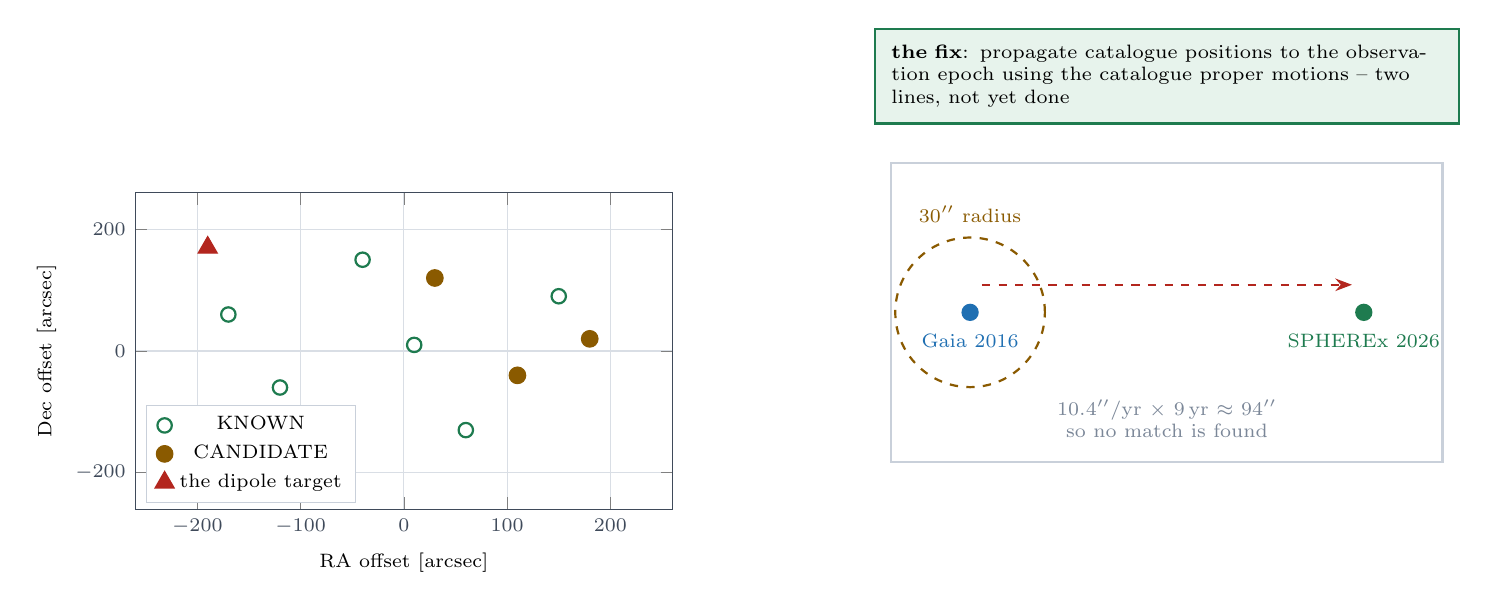
\begin{tikzpicture}[font=\footnotesize]
  \begin{scope}
    \begin{axis}[width=8.4cm,height=5.6cm,
      xlabel={RA offset [arcsec]},ylabel={Dec offset [arcsec]},
      xlabel style={font=\scriptsize},ylabel style={font=\scriptsize},
      xmin=-260,xmax=260,ymin=-260,ymax=260,
      grid=both,grid style={rule!70},axis line style={slate},
      tick label style={font=\scriptsize,text=slate},
      legend style={font=\scriptsize,draw=rule,at={(0.02,0.02)},anchor=south west}]
    \addplot[only marks,mark=o,mark size=2.6pt,good,line width=0.8pt] coordinates {
      (-120,-60) (60,-130) (-40,150) (150,90) (10,10) (-170,60)};
    \addlegendentry{KNOWN}
    \addplot[only marks,mark=*,mark size=3.0pt,warn] coordinates {(-60,-160) (110,-40) (30,120) (-140,-140) (180,20)};
    \addlegendentry{CANDIDATE}
    \addplot[only marks,mark=triangle*,mark size=4.0pt,bad] coordinates {(-190,170)};
    \addlegendentry{the dipole target}
    \end{axis}
  \end{scope}
  \begin{scope}[shift={(9.6,0.6)}]
    \draw[rule,thick,fill=white] (0,0) rectangle (7.0,3.8);
    \fill[accent] (1.0,1.9) circle (0.11);
    \node[font=\scriptsize,text=accent,below] at (1.0,1.74) {Gaia 2016};
    \fill[good] (6.0,1.9) circle (0.11);
    \node[font=\scriptsize,text=good,below] at (6.0,1.74) {SPHEREx 2026};
    \draw[warn,dashed,thick] (1.0,1.9) circle (0.95);
    \node[font=\scriptsize,text=warn,above] at (1.0,2.92) {$30\arcsec$ radius};
    \draw[-{Stealth[length=6pt]},thick,bad,dashed] (1.15,2.25) -- (5.85,2.25);
    \node[font=\scriptsize,text=muted,align=center] at (3.5,0.55) {$10.4\arcsec$/yr $\times$ 9\,yr $\approx$ 94\arcsec\\ so no match is found};
    \node[draw=good,thick,fill=good2,align=left,inner sep=6pt,text width=7.0cm,font=\scriptsize] at (3.5,4.9)
      {\textbf{the fix}: propagate catalogue positions to the observation epoch using the catalogue proper motions -- two lines, not yet done};
  \end{scope}
\end{tikzpicture}}

\textbf{Spoken script.} What are the seventeen? Care is needed here, because this is where a project like
this usually gets oversold. The scatter on the left is a typical field: hollow circles are detections the
catalogues explain, filled dots are the unexplained ones, and the triangle is the target itself.\par
Most of the seventeen are simply positions where a five-sigma change has no catalogue source within
thirty arcseconds. Five of them are in WISE 0855, the field with the fewest catalogue sources per unit
noise -- exactly what you would expect if the candidate rate tracks catalogue density rather than
astrophysics. And the single most significant detection in the whole sample, Barnard's Star at fifty-seven
sigma, is itself a mislabel for the epoch reason on the right: Gaia's position is from 2016, this image
is from 2026, the star has moved ninety-four arcseconds, and nothing matches.\par
So the result actually being claimed is narrow: seventeen positions where a five-sigma change is
unexplained by three catalogues. Not seventeen new objects. The word on the slide is unexplained.

\newpage
% -------------------------------------------------------------- SLIDE 22 ---
\slidehead{22}{Live demonstration}{1:30}

\textbf{On the slide.}
\begin{itemize}[leftmargin=1.4em,itemsep=2pt,topsep=2pt]
\item Open \code{site/index.html} -- already loaded in a second tab, 100\% zoom
\item \textbf{1} pick Barnard's Star, point at the dipole, hover it \;\textbullet\; \textbf{2} click it: verdict, SNR, proper motion
\item \textbf{3} switch layers: co-add, difference, significance
\item \textbf{4} all-sky view, then the Crab Nebula (10 detections, all KNOWN)
\item \textbf{5} recovery grid on the current field \;\textbullet\; \textbf{6} the Guide tab
\end{itemize}

\textbf{Figure / diagram.} A map of the screen with the six numbered callouts sitting in the gutters
beside the exact controls used, so nothing has to be hunted for on stage.

\figbox{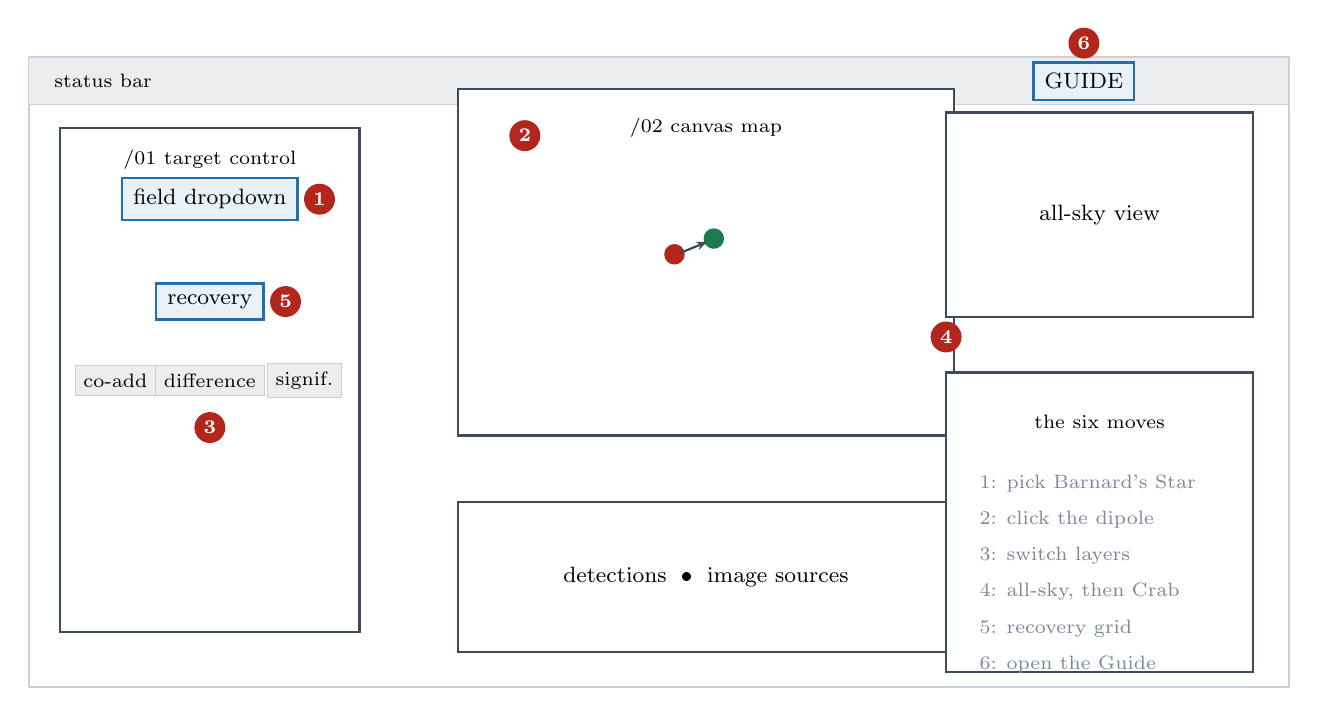
\begin{tikzpicture}[font=\footnotesize,
  cb/.style={circle,draw=bad,thick,fill=bad,text=white,inner sep=1.4pt,font=\scriptsize\bfseries},
  pan/.style={draw=slate,thick,fill=white,align=center,inner sep=4pt},
  chip/.style={draw=accent,thick,fill=accent2,align=center,inner sep=4pt}]
  \draw[rule,thick,fill=white] (0,0) rectangle (16.0,8.0);
  % top bar
  \draw[rule,fill=slate!10] (0,7.4) rectangle (16.0,8.0);
  \node[anchor=west,font=\scriptsize] at (0.2,7.7) {status bar};
  \node[chip] (guide) at (13.4,7.7) {GUIDE};
  \node[cb,above=1pt of guide] {6};
  % left column
  \node[pan,minimum width=3.8cm,minimum height=6.4cm] (left) at (2.3,3.9) {};
  \node[anchor=north,font=\scriptsize] at (2.3,6.95) {/01 target control};
  \node[chip] (drop) at (2.3,6.2) {field dropdown};
  \node[cb,right=2pt of drop] {1};
  \node[chip,minimum width=1.0cm] (rec) at (2.3,4.9) {recovery};
  \node[cb,right=2pt of rec] {5};
  \foreach \x/\lab in {1.1/{co-add},2.3/{difference},3.5/{signif.}}{\node[draw=rule,fill=slate!10,inner sep=3pt,font=\scriptsize] at (\x,3.9) {\lab};}
  \node[cb] at (2.3,3.30) {3};
  % map
  \node[pan,minimum width=6.3cm,minimum height=4.4cm] (map) at (8.6,5.4) {};
  \node[anchor=north,font=\scriptsize] at (8.6,7.35) {/02 canvas map};
  \fill[bad] (8.2,5.5) circle (0.13);
  \fill[good] (8.7,5.7) circle (0.13);
  \draw[-{Stealth[length=4pt]},thick,slate] (8.28,5.52) -- (8.62,5.66);
  \node[cb,above=6pt] at (6.3,6.6) {2};
  % tables
  \node[pan,minimum width=6.3cm,minimum height=1.9cm] (tab) at (8.6,1.4) {detections \;\textbullet\; image sources};
  % all-sky
  \node[pan,minimum width=3.9cm,minimum height=2.6cm] (sky) at (13.6,6.0) {all-sky view};
  \node[cb] at (11.65,4.45) {4};
  % steps
  \node[pan,minimum width=3.9cm,minimum height=3.8cm] (steps) at (13.6,2.1) {};
  \node[anchor=north,font=\scriptsize] at (13.6,3.58) {the six moves};
  \foreach \i/\txt in {1/{pick Barnard's Star},2/{click the dipole},3/{switch layers},4/{all-sky, then Crab},5/{recovery grid},6/{open the Guide}}{\node[anchor=west,font=\scriptsize,text=muted] at (11.95,3.05-\i*0.46) {\i: \txt};}
\end{tikzpicture}}

\textbf{Spoken script.} I would like to show this working rather than describe it, so the site is open in
the second tab. This is the static version, no server, so everything you are about to see is pre-computed
JSON being drawn by the browser.\par
First, Barnard's Star, which is the demo I would recommend to anyone. The map shows the significance of
the difference between two visits. Point at that bright pair in the middle -- a dipole, the star's old
position in red, its new one in green -- and the tooltip gives the verdict, the significance and the
catalogues that match. Click it and the verdict panel opens: this is the fifty-seven-sigma detection, a
proper motion around twenty-five arcseconds a year, and no catalogue match, for the epoch reason from
slide fourteen.\par
Now the layer switch: co-add, then difference, then significance -- the whole chain, visible one step at
a time. Over to the all-sky view, where every field is a thumbnail; I will pick the Crab, which gives ten
detections and all ten explained, because that is the contrast I want you to see. Finally the recovery
grid for the field, which is the completeness matrix, and the Guide tab, which is what a visitor sees
before anyone explains anything to them.\par
If the laptop misbehaves, the fallback is the same content in the report -- figures three, six and seven
-- and I will move on rather than debug in front of you.

\newpage
% -------------------------------------------------------------- SLIDE 23 ---
\slidehead{23}{Conclusion, contributions, and questions}{0:50}

\textbf{On the slide.}
\begin{itemize}[leftmargin=1.4em,itemsep=2pt,topsep=2pt]
\item \textbf{Works}: ZOGY on masked co-adds gives a calibrated $5\sigma$ map, morphology separates
      movers from variables, triage explains 81\% of detections
\item \textbf{Honest}: four fields return nothing, completeness is unmeasured, one candidate is our own bug
\item \textbf{Next}: local-noise injection, proper-motion propagation, an empirical PSF, all 102 bands
\item Artefact: six stages, the derived JSON, a static site, and a guide for non-specialists
\end{itemize}

\textbf{Figure / diagram.} Three pillars -- works, honest, next -- with the artefact listed underneath and
a compact reference strip at the bottom.

\figbox{\begin{tikzpicture}[font=\footnotesize,
  p/.style={draw=rule,thick,fill=white,align=center,inner sep=7pt,text width=4.6cm}]
  \node[p] (a) at (2.6,2.6) {\Large\bfseries WORKS\\[5pt] \footnotesize calibrated $5\sigma$ via ZOGY\\
      81\% of detections explained\\ movers told from variables};
  \node[p] (b) at (8.4,2.6) {\Large\bfseries HONEST\\[5pt] \footnotesize four empty fields reported\\
      completeness not invented\\ our own bug diagnosed};
  \node[p] (c) at (14.2,2.6) {\Large\bfseries NEXT\\[5pt] \footnotesize local-noise injection\\
      proper-motion propagation\\ empirical PSF, all 102 bands};
  \node[draw=accent,thick,fill=accent2,align=center,inner sep=6pt,text width=16.2cm,font=\footnotesize] at (8.4,-0.2)
    {artefact: 6\,154 lines \;\textbullet\; \code{site/index.html}, 28\,MB, no server \;\textbullet\;
     every number traceable to a Level-2 file at IRSA \;\textbullet\; 33-page report};
  \node[align=left,text width=16.2cm,font=\scriptsize,text=muted,anchor=north west] at (0.3,-0.9)
    {\textbf{references:} Alard \& Lupton 1998 \;\textbullet\; Bramich 2008 \;\textbullet\;
     Zackay, Ofek \& Gal-Yam 2016 \;\textbullet\; Hu et al.\ 2022 (SFFT) \;\textbullet\;
     ZTF and DES pipelines, and the broker literature (ANTARES, ALeRCE, Lasair) \;\textbullet\;
     Gaia DR3, AllWISE, AAVSO VSX \;\textbullet\; SPHEREx mission and IRSA documentation};
\end{tikzpicture}}

\textbf{Spoken script.} To close, three statements, and then questions.\par
It works: proper subtraction on masked co-adds gives a significance map whose threshold means something,
the morphology separates movers from variables wherever the displacement exceeds the PSF, and catalogue
triage explains four fifths of what the pipeline finds.\par
It is honest: four fields came back empty and the deck says so, the completeness is still unmeasured
rather than invented, and the single most significant detection in the sample is a bug found in my own
triage and described rather than hidden.\par
And the next three changes are small, and each one converts a caveat into a number: inject at the image
level with local noise, propagate catalogue proper motions before matching, and use an empirical PSF per
detector. Everything is in the repository -- the six stages, the derived JSON, the static site, and a
guide written for someone who has never seen an astronomical image. Thank you; I am happy to take
questions.

\newpage
% -------------------------------------------------------------- BACKUP -----
{\large\bfseries Backup: five questions and the pre-flight checklist}\par
\vspace{2pt}\hrule height 0.9pt\vspace{8pt}

\textbf{Questions you are most likely to be asked.}
\begin{description}[leftmargin=1.6em,itemsep=4pt]
\item[``Why only two or three bands, and not all 102?''] Cost: a hundred and two cutouts per epoch per
field is roughly 500\,MB and seventy minutes of archive time, \emph{per field}. Subtraction does not need
the extra bands; the spectral indices do, and that is the first item on the next-steps list.
\item[``Is thirty arcseconds not far too generous a match radius?''] For astrometry, yes. For vetoing it
is deliberate: a loose radius biases towards KNOWN, which is the conservative direction. The alternative
inflates the candidate list and flatters the result.
\item[``What is the real false-positive rate?''] Predicted 0.018 pixels per frame at $5\sigma$; the
observed detections are tens of sigma above that floor, so the map is not noise-dominated. No measured
rate is quoted, because completeness is unmeasured.
\item[``Could this scale to the whole sky?''] The CPU could: six seconds per field times 1.8 million
nine-arcminute fields is about 125 days on one core. The archive is the bottleneck, which is why the
design caches aggressively and pre-renders.
\item[``Why ZOGY rather than SFFT?''] ZOGY is closed form and its null distribution is analytic, which is
what makes the false-positive budget explicit -- the argument on slide twelve. SFFT would be the better
choice for an undersampled space PSF, and is listed as future work.
\end{description}

\vspace{4pt}
\textbf{Pre-flight checklist, five minutes before.}
\begin{itemize}[leftmargin=1.5em,itemsep=2pt]
\item Two browser tabs: \code{site/index.html} (static, offline-safe) and, if the network is good, the
local API on \code{localhost:8000} for the live fetch.
\item Zoom 100\%, one field already loaded -- Barnard's Star -- so the demo does not start on a spinner.
\item A screen recording of the demo on the desktop, as the fallback file.
\item This document open at page 23, the demo map, so the callouts match the screen.
\item Numbers on the tip of the tongue: 18 fields, 128 cutouts, 88 detections, 71 explained,
17 unexplained, 4 empty fields, 0.018 false pixels per frame.
\end{itemize}

\end{document}
